%% (Master) Thesis template
% Template version used: v1.4
%
% Largely adapted from Adrian Nievergelt's template for the ADPS
% (lecture notes) project.

\PassOptionsToPackage{dvipsnames}{xcolor}

%% We use the memoir class because it offers many easy to use features.
\documentclass[11pt,a4paper,titlepage]{memoir}

%% Packages
%% ========

%% LaTeX Font encoding -- DO NOT CHANGE
\usepackage[OT1]{fontenc}

%% Babel provides support for languages.  'english' uses British
%% English hyphenation and text snippets like "Figure" and
%% "Theorem". Use the option 'ngerman' if your document is in German.
%% Use 'american' for American English.  Note that if you change this,
%% the next LaTeX run may show spurious errors.  Simply run it again.
%% If they persist, remove the .aux file and try again.
\usepackage[american]{babel}

%% Input encoding 'utf8'. In some cases you might need 'utf8x' for
%% extra symbols. Not all editors, especially on Windows, are UTF-8
%% capable, so you may want to use 'latin1' instead.
\usepackage[utf8]{inputenc}

%% This changes default fonts for both text and math mode to use Herman Zapfs
%% excellent Palatino font.  Do not change this.
\usepackage[sc]{mathpazo}

%% The AMS-LaTeX extensions for mathematical typesetting.  Do not
%% remove.
\usepackage{amsmath,amssymb,amsfonts,mathrsfs}

%% NTheorem is a reimplementation of the AMS Theorem package. This
%% will allow us to typeset theorems like examples, proofs and
%% similar.  Do not remove.
%% NOTE: Must be loaded AFTER amsmath, or the \qed placement will
%% break
\usepackage[amsmath,thmmarks]{ntheorem}

%% LaTeX' own graphics handling
\usepackage{graphicx}
\graphicspath{{figures/}} %tell package where to find graphics


%% We unfortunately need this for the Rules chapter.  Remove it
%% afterwards; or at least NEVER use its underlining features.
\usepackage{soul}

%% This allows you to add .pdf files. It is used to add the
%% declaration of originality.
\usepackage{pdfpages}

\usepackage{xspace}

\usepackage{capt-of}

\usepackage{float}

\usepackage[section]{placeins}

\usepackage{subfig}

\usepackage[square, comma, sort&compress, numbers]{natbib}
%% Some more packages that you may want to use.  Have a look at the
%% file, and consult the package docs for each.
%% See the TeXed file for more explanations

%% [OPT] Multi-rowed cells in tabulars
%\usepackage{multirow}

%% [REC] Intelligent cross reference package. This allows for nice
%% combined references that include the reference and a hint to where
%% to look for it.
\usepackage{varioref}

%% [OPT] Easily changeable quotes with \enquote{Text}
%\usepackage[german=swiss]{csquotes}

%% [REC] Format dates and time depending on locale
\usepackage{datetime}

%% [OPT] Provides a \cancel{} command to stroke through mathematics.
%\usepackage{cancel}

%% [NEED] This allows for additional typesetting tools in mathmode.
%% See its excellent documentation.
\usepackage{mathtools}

%% [ADV] Conditional commands
%\usepackage{ifthen}

%% [OPT] Manual large braces or other delimiters.
%\usepackage{bigdelim, bigstrut}

%% [REC] Alternate vector arrows. Use the command \vv{} to get scaled
%% vector arrows.
\usepackage[h]{esvect}

%% [NEED] Some extensions to tabulars and array environments.
\usepackage{array}

%% [OPT] Postscript support via pstricks graphics package. Very
%% diverse applications.
%\usepackage{pstricks,pst-all}

%% [?] This seems to allow us to define some additional counters.
%\usepackage{etex}

%% [ADV] XY-Pic to typeset some matrix-style graphics
%\usepackage[all]{xy}

%% [OPT] This is needed to generate an index at the end of the
%% document.
%\usepackage{makeidx}

%% [OPT] Fancy package for source code listings.  The template text
%% needs it for some LaTeX snippets; remove/adapt the \lstset when you
%% remove the template content.
%% Settings for code listings
\usepackage{listings}
\usepackage{listings-golang}
\lstset{ % add your own preferences
	frame=single,
	basicstyle=\footnotesize,
	keywordstyle=\color{violet},
	commentstyle=\color{OliveGreen},
	numbers=left,
	numbersep=5pt,
	showstringspaces=false, 
	stringstyle=\color{magenta},
	tabsize=4,
	language=golang
}

\lstdefinelanguage{yaml}
{
 morekeywords=[1]{mysql_db,mysql_pass,apt,name,password,host,login_password,mysql_db,mysql_user,with_items,jobs,build,docker,image,environment,MYSQL_ROOT_PASSWORD,MYSQL_DATABASE,steps,run,command,working_directory,version},
	sensitive=true,
	morestring=[b]",
%	morecomment=[l]:,
}

\lstset{ % add your own preferences
	frame=single,
	basicstyle=\footnotesize,
	keywordstyle=\color{blue},
	commentstyle=\color{OliveGreen},
	moredelim = [l][\functionColonHighlight]{:}{ljl}
	numbers=left,
	numbersep=5pt,
	showstringspaces=false, 
	stringstyle=\color{magenta},
	tabsize=4,
	language=yaml
}

\newcommand{\functionColonHighlight}[1]{\bfseries\textcolor{blue}{:} \textcolor{magenta}{\mdseries #1}(}



%% [REC] Fancy character protrusion.  Must be loaded after all fonts.
\usepackage[activate]{pdfcprot}

%% [REC] Nicer tables.  Read the excellent documentation.
\usepackage{booktabs}


%% Our layout configuration.  DO NOT CHANGE.
%% Memoir layout setup

%% NOTE: You are strongly advised not to change any of them unless you
%% know what you are doing.  These settings strongly interact in the
%% final look of the document.

% Dependencies
\usepackage{ETHlogo}

% Turn extra space before chapter headings off.
\setlength{\beforechapskip}{0pt}

\nonzeroparskip
\parindent=0pt
\defaultlists

% Chapter style redefinition
\makeatletter

\if@twoside
  \pagestyle{Ruled}
  \copypagestyle{chapter}{Ruled}
\else
  \pagestyle{ruled}
  \copypagestyle{chapter}{ruled}
\fi
\makeoddhead{chapter}{}{}{}
\makeevenhead{chapter}{}{}{}
\makeheadrule{chapter}{\textwidth}{0pt}
\copypagestyle{abstract}{empty}

\makechapterstyle{bianchimod}{%
  \chapterstyle{default}
  \renewcommand*{\chapnamefont}{\normalfont\Large\sffamily}
  \renewcommand*{\chapnumfont}{\normalfont\Large\sffamily}
  \renewcommand*{\printchaptername}{%
    \chapnamefont\centering\@chapapp}
  \renewcommand*{\printchapternum}{\chapnumfont {\thechapter}}
  \renewcommand*{\chaptitlefont}{\normalfont\huge\sffamily}
  \renewcommand*{\printchaptertitle}[1]{%
    \hrule\vskip\onelineskip \centering \chaptitlefont\textbf{\vphantom{gyM}##1}\par}
  \renewcommand*{\afterchaptertitle}{\vskip\onelineskip \hrule\vskip
    \afterchapskip}
  \renewcommand*{\printchapternonum}{%
    \vphantom{\chapnumfont {9}}\afterchapternum}}

% Use the newly defined style
\chapterstyle{bianchimod}

\setsecheadstyle{\Large\bfseries\sffamily}
\setsubsecheadstyle{\large\bfseries\sffamily}
\setsubsubsecheadstyle{\bfseries\sffamily}
\setparaheadstyle{\normalsize\bfseries\sffamily}
\setsubparaheadstyle{\normalsize\itshape\sffamily}
\setsubparaindent{0pt}

% Set captions to a more separated style for clearness
\captionnamefont{\sffamily\bfseries\footnotesize}
\captiontitlefont{\sffamily\footnotesize}
\setlength{\intextsep}{16pt}
\setlength{\belowcaptionskip}{1pt}

% Set section and TOC numbering depth to subsection
\setsecnumdepth{subsection}
\settocdepth{subsection}

%% Titlepage adjustments
\pretitle{\vspace{0pt plus 0.7fill}\begin{center}\HUGE\sffamily\bfseries}
\posttitle{\end{center}\par}
\preauthor{\par\begin{center}\let\and\\\Large\sffamily}
\postauthor{\end{center}}
\predate{\par\begin{center}\Large\sffamily}
\postdate{\end{center}}

\def\@advisors{}
\newcommand{\advisors}[1]{\def\@advisors{#1}}
\def\@department{}
\newcommand{\department}[1]{\def\@department{#1}}
\def\@thesistype{}
\newcommand{\thesistype}[1]{\def\@thesistype{#1}}

\renewcommand{\maketitlehooka}{\noindent\ETHlogo[2in]}

\renewcommand{\maketitlehookb}{\vspace{1in}%
  \par\begin{center}\Large\sffamily\@thesistype\end{center}}

\renewcommand{\maketitlehookd}{%
  \vfill\par
  \begin{flushright}
    \sffamily
    \@advisors\par
    \@department, ETH Z\"urich
  \end{flushright}
}

\checkandfixthelayout

\setlength{\droptitle}{-48pt}

\makeatother

% This defines how theorems should look. Best leave as is.
\theoremstyle{plain}
\setlength\theorempostskipamount{0pt}

%%% Local Variables:
%%% mode: latex
%%% TeX-master: "thesis"
%%% End:


%% Theorem environments.  You will have to adapt this for a German
%% thesis.
%% Theorem-like environments

%% This can be changed according to language. You can comment out the ones you
%% don't need.

\numberwithin{equation}{chapter}

%% German theorems
%\newtheorem{satz}{Satz}[chapter]
%\newtheorem{beispiel}[satz]{Beispiel}
%\newtheorem{bemerkung}[satz]{Bemerkung}
%\newtheorem{korrolar}[satz]{Korrolar}
%\newtheorem{definition}[satz]{Definition}
%\newtheorem{lemma}[satz]{Lemma}
%\newtheorem{proposition}[satz]{Proposition}

%% English variants
\newtheorem{theorem}{Theorem}[chapter]
\newtheorem{example}[theorem]{Example}
\newtheorem{remark}[theorem]{Remark}
\newtheorem{corollary}[theorem]{Corollary}
\newtheorem{definition}[theorem]{Definition}
\newtheorem{lemma}[theorem]{Lemma}
\newtheorem{proposition}[theorem]{Proposition}

%% Proof environment with a small square as a "qed" symbol
\theoremstyle{nonumberplain}
\theorembodyfont{\normalfont}
\theoremsymbol{\ensuremath{\square}}
\newtheorem{proof}{Proof}
%\newtheorem{beweis}{Beweis}


%% Helpful macros.
%% Custom commands
%% ===============

%% Special characters for number sets, e.g. real or complex numbers.
\newcommand{\C}{\mathbb{C}}
\newcommand{\K}{\mathbb{K}}
\newcommand{\N}{\mathbb{N}}
\newcommand{\Q}{\mathbb{Q}}
\newcommand{\R}{\mathbb{R}}
\newcommand{\Z}{\mathbb{Z}}
\newcommand{\X}{\mathbb{X}}

%% Fixed/scaling delimiter examples (see mathtools documentation)
\DeclarePairedDelimiter\abs{\lvert}{\rvert}
\DeclarePairedDelimiter\norm{\lVert}{\rVert}

%% Use the alternative epsilon per default and define the old one as \oldepsilon
\let\oldepsilon\epsilon
\renewcommand{\epsilon}{\ensuremath\varepsilon}

%% Also set the alternate phi as default.
\let\oldphi\phi
\renewcommand{\phi}{\ensuremath{\varphi}}

\newcommand{\lee}{\textit{SCIONLab Experimentation Environment}\xspace}
\newcommand{\lcs}{\textit{SCIONLab Coordination Service}\xspace}
\newcommand{\lmi}{\textit{Local Management Service}\xspace}
\newcommand{\cords}{\textit{Coordination Service}\xspace}
\newcommand{\fnurl}[2]{\href{#2}{#1}\footnote{\url{#2}}\xspace}
\newcommand{\fnote}[2]{#1\footnote{#2}}\xspace
\newcommand{\fnoteurl}[3]{\href{#2}{#1}\footnote{{#3:} \url{#2}}\xspace}
\newcommand{\code}[1]{\colorbox{lightgray}{\textit{"#1"}}\xspace}
\newif\ifcomment
\newcommand{\cmnt}[1]{\ifcomment {\color{orange}{#1}} \fi}


\newcommand{\customtoday}{\ifcase \month \or January \or February \or March \or %
	April \or May \or June \or July \or August \or September \or October \or November \or %
	December \fi \number \day, \number \year} 


%% Make document internal hyperlinks wherever possible. (TOC, references)
%% This MUST be loaded after varioref, which is loaded in 'extrapackages'
%% above.  We just load it last to be safe.
\usepackage[linkcolor=black,colorlinks=true,citecolor=black,filecolor=black]{hyperref}

%% Document information
%% ====================

%%render comments
\commentfalse

\title{\LARGE{The Danger of Overthinking: Failure of Reasoning Models on SWE-Bench}}
\author{Alex Cuadron}
\thesistype{Master Thesis}
\advisors{Advisors: Prof.\ Dr.\ Joey Velez-Ginorio, Dr.\ Dacheng Li}
\department{Department of Computer Science}
\date{March 15, 2024}

\begin{document}

\frontmatter

%% Title page is autogenerated from document information above.  DO
%% NOT CHANGE.
\begin{titlingpage}
        \calccentering{\unitlength}
        \begin{adjustwidth*}{\unitlength-24pt}{-\unitlength-24pt}
                \maketitle
        \end{adjustwidth*}
\end{titlingpage}

%% The abstract of your thesis.  Edit the file as needed.
\begin{abstract}
        Large Reasoning Models (LRMs) represent a breakthrough in AI problem-solving capabilities, but their effectiveness in interactive environments may be limited. This thesis introduces and analyzes \textbf{overthinking} in LRMs—a phenomenon where models favor extended internal reasoning chains over environmental interaction. Through experiments on software engineering tasks using SWE Bench Verified, we observe three recurring patterns: \textit{Analysis Paralysis, Rogue Actions, and Premature Disengagement}. We propose a framework to study these behaviors, which correlates with human expert assessments, and analyze \textbf{3,908 trajectories}. We observe that higher overthinking scores correlate with decreased performance, with reasoning models exhibiting stronger tendencies toward overthinking compared to non-reasoning models. Our analysis reveals that simple solutions—such as selecting solutions with lower overthinking scores—can \textbf{improve model performance by 25\% while decreasing computational costs by 43\%}. Based on these findings, we suggest promising directions for mitigating overthinking through native function-calling capabilities and selective reinforcement learning, potentially offering a path to better balance reasoning and environmental interaction. To facilitate further research in this direction, we open-source our evaluation framework and dataset.
\end{abstract}

\addcontentsline{toc}{section}{Abstract}
\newpage

%% The acknowledgements
\renewcommand{\abstractname}{Acknowledgments}
\begin{abstract}
	First and foremost, I would like to thank Prof. Dr. Adrian Perrig for providing me the opportunity of working
	on this fascinating project. His continued support is very appreciated.

	I would like to express my sincere gratitude to Dr. Jonghoon Kwon and Patrick Bamert for the
	many discussions and valuable insights. Without their help, this thesis would not have been possible.

	Lastly, my special thank goes to my family and friends for their unconditional support throughout
	my studies.
\end{abstract}

\addcontentsline{toc}{section}{Acknowledgments}
\newpage

%% Citing the paper
\renewcommand{\abstractname}{Preface}
\begin{abstract}
	The work done in this thesis has additionally been submitted as research
	paper~\cite{kwon2020Mondrian}. At the time of writing, the manuscript has
	been submitted and is undergoing review.
	This thesis aims to expand on the paper, giving deeper insights into the different aspects of \name.
\end{abstract}

\addcontentsline{toc}{section}{Preface}

%% TOC with the proper setup, do not change.
\cleartorecto
\tableofcontents
\mainmatter

%% Your real content!
\chapter{Introduction}
\label{intro}

Large Reasoning Models (LRMs) represent a breakthrough in AI problem-solving capabilities, yet their effectiveness in interactive environments remains poorly understood. This thesis introduces and analyzes the phenomenon of \textbf{overthinking} in LRMs - a tendency where models prioritize elaborate internal simulations of potential actions over gathering actual environmental feedback. Through extensive experiments on software engineering tasks using SWE Bench Verified, we develop a systematic framework to quantify overthinking behavior on a 0-10 scale, measuring how models balance internal reasoning chains against environmental interaction.

\begin{figure}[t]
    \centering
    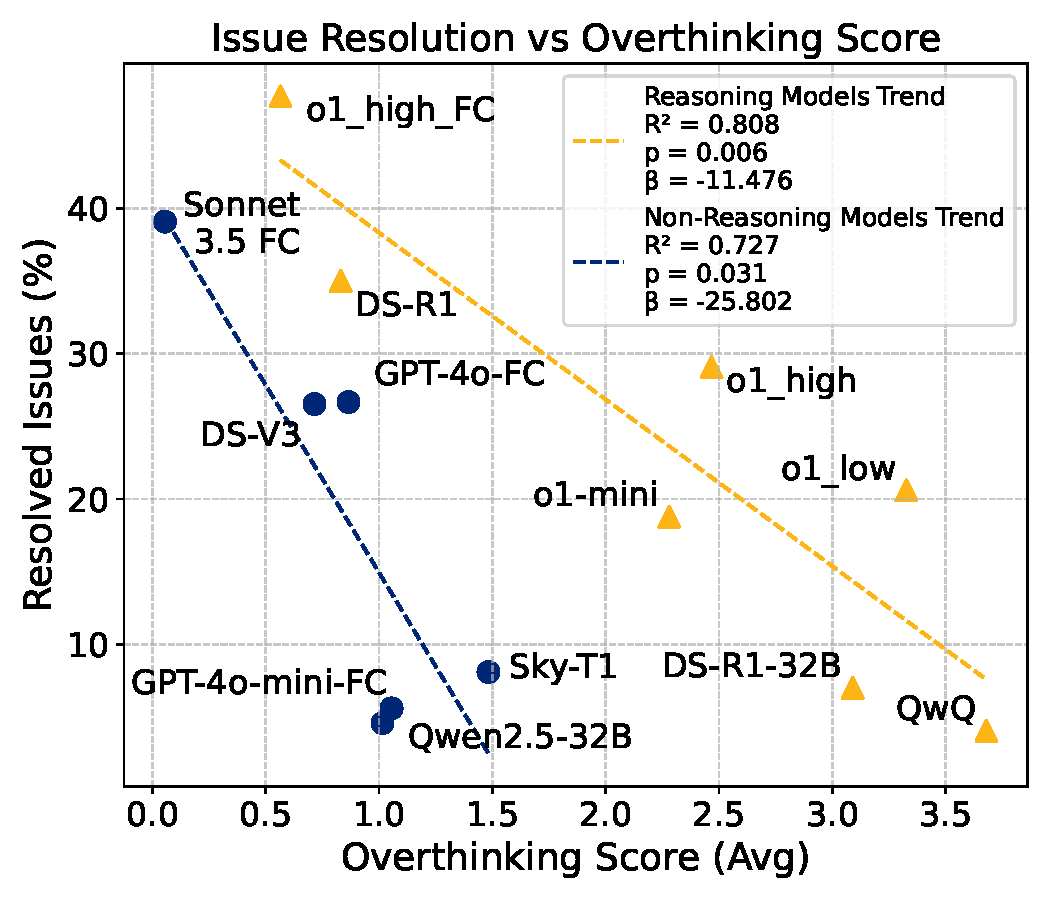
\includegraphics[width=1\linewidth]{model_analysis_combined.pdf}
    \caption{Higher overthinking scores (tendency to favor internal reasoning over environmental feedback) correlate with lower issue resolution rates across all models. Reasoning models exhibit consistently higher overthinking tendencies, suggesting that excessive reliance on internal simulation impairs task performance. Model nomenclature: "FC" indicates native function calling capability, "DS" represents DeepSeek models, and suffixes o1\_high and o1\_low denote models with reasoning effort set to high and low respectively.}
    \label{fig:figure1}
\end{figure}

\begin{figure}[t]
    \centering
    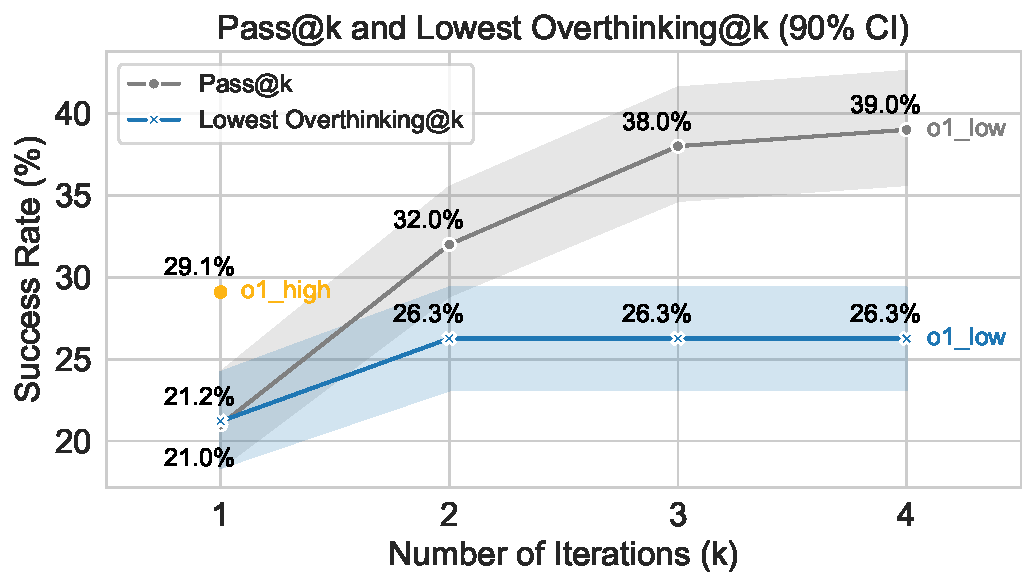
\includegraphics[width=1\linewidth]{pass_at_k_plot.pdf}
    \caption{Pass@k performance for SWE Bench Verified when selecting responses based on overthinking scores. By choosing solutions with minimal overthinking from multiple runs of o1 with low reasoning effort, we achieve performance comparable to high reasoning effort configurations at substantially lower computational cost. The flattening curve suggests diminishing returns from additional iterations, with detailed performance metrics provided in \cref{tab:o1_model_comparison}. The confidence intervals (CI) showcased were computed using Wilson score.}
    \label{fig:figure2}
\end{figure}

Analysis of \textbf{3,908 trajectories} reveals that overthinking significantly impairs model performance, with strong negative correlations between overthinking scores and issue resolution capabilities (R² = 0.808, p = 0.006 for reasoning models). Notably, LRMs exhibit higher overthinking scores (2.320 ± 1.120) compared to non-reasoning models (0.865 ± 0.432, p = 0.019). Based on our findings, we propose that integrating native function-calling capabilities during training may help models better balance reasoning and action.

\section{The Rise of Large Reasoning Models}
LRMs, defined as LLMs leveraging reinforcement learning techniques for train-time scaling, represent a breakthrough in AI reasoning capabilities. These models are fundamentally built on the principle that allocating more computational resources at test-time enables deeper reasoning. This approach has proven remarkably effective: by dedicating significant compute to deliberate reasoning steps, these models achieve unprecedented performance through extended chain-of-thought reasoning, systematic exploration of solution strategies, and rigorous self-verification. However, this extended focus on internal reasoning depth raises important questions about how these models balance internal deliberation with action in interactive environments.

\section{The Challenge of Agentic Environments}
While traditional AI defined agents broadly as entities that perceive and act upon their environment, the LLM era has evolved toward viewing agency as a spectrum of capabilities. Systems are considered more agentic based on three key factors:
\begin{itemize}
    \item Their ability to handle complex environments and pursue goals autonomously
    \item Their capacity to act with minimal supervision through natural language interfaces
    \item Their use of advanced design patterns such as tool utilization and dynamic planning
\end{itemize}

These principles have been extensively applied to software engineering tasks, particularly in solving real-world GitHub issues, where numerous research efforts have explored different agent architectures with varying degrees of success. While these efforts have advanced our understanding of AI agents in software engineering, they have not specifically examined how LRMs' unique reasoning capabilities affect their performance in agentic environments—a critical gap our work addresses.

\section{The Reasoning-Action Dilemma}
We observe that, in agentic decision-making tasks, LRMs constantly face the \emph{Reasoning–Action Dilemma} where they must navigate a fundamental trade-off between:
\begin{itemize}
    \item \textbf{Direct interaction with the environment}, where the model executes actions and receives feedback
    \item \textbf{Internal reasoning}, where the model reasons over hypothetical outcomes before committing to an action
\end{itemize}

Ideally, an LRM should balance reasoning and action by using internal simulation to refine its choices while leveraging real-world feedback to correct errors. For instance, when debugging a failing test case, a well-balanced model would hypothesize potential issues yet still execute the test opportunely to collect concrete failure signals.

\section{Contributions}
This thesis makes several key contributions to understanding and addressing the overthinking phenomenon in LRMs:

\begin{enumerate}
    \item We introduce and formalize the concept of overthinking in LRMs, distinguishing it from related phenomena like hallucination
    \item We develop a systematic framework for quantifying overthinking behavior, validated against human expert assessments
    \item We provide extensive empirical evidence of overthinking patterns across different model architectures through analysis of over 3,908 model responses
    \item We demonstrate practical solutions that can improve model performance by 25\% while reducing computational costs by 43\%
\end{enumerate}

\section{Thesis Structure}
The remainder of this thesis is organized as follows:

\begin{itemize}
    \item Chapter \ref{background} provides essential background on LRMs and agentic environments
    \item Chapter \ref{overthinking} introduces our framework for diagnosing and quantifying overthinking
    \item Chapter \ref{evaluation} presents our experimental results and analysis
    \item Chapter \ref{discussion} discusses implications and potential solutions
    \item Chapter \ref{conclusion} summarizes our findings and suggests future research directions
\end{itemize}

To facilitate further research in this direction, we open-source our evaluation framework and comprehensive dataset of annotated model trajectories.
 % Introduction
\chapter{Background}
\label{background}

Using a case study we explore how network zoning is realized in modern enterprise networks, and later we derive the main challenges we confront.

\section{Case Study}
\label{sec:casestudy}

\begin{figure}[htb]
	\begin{center}
		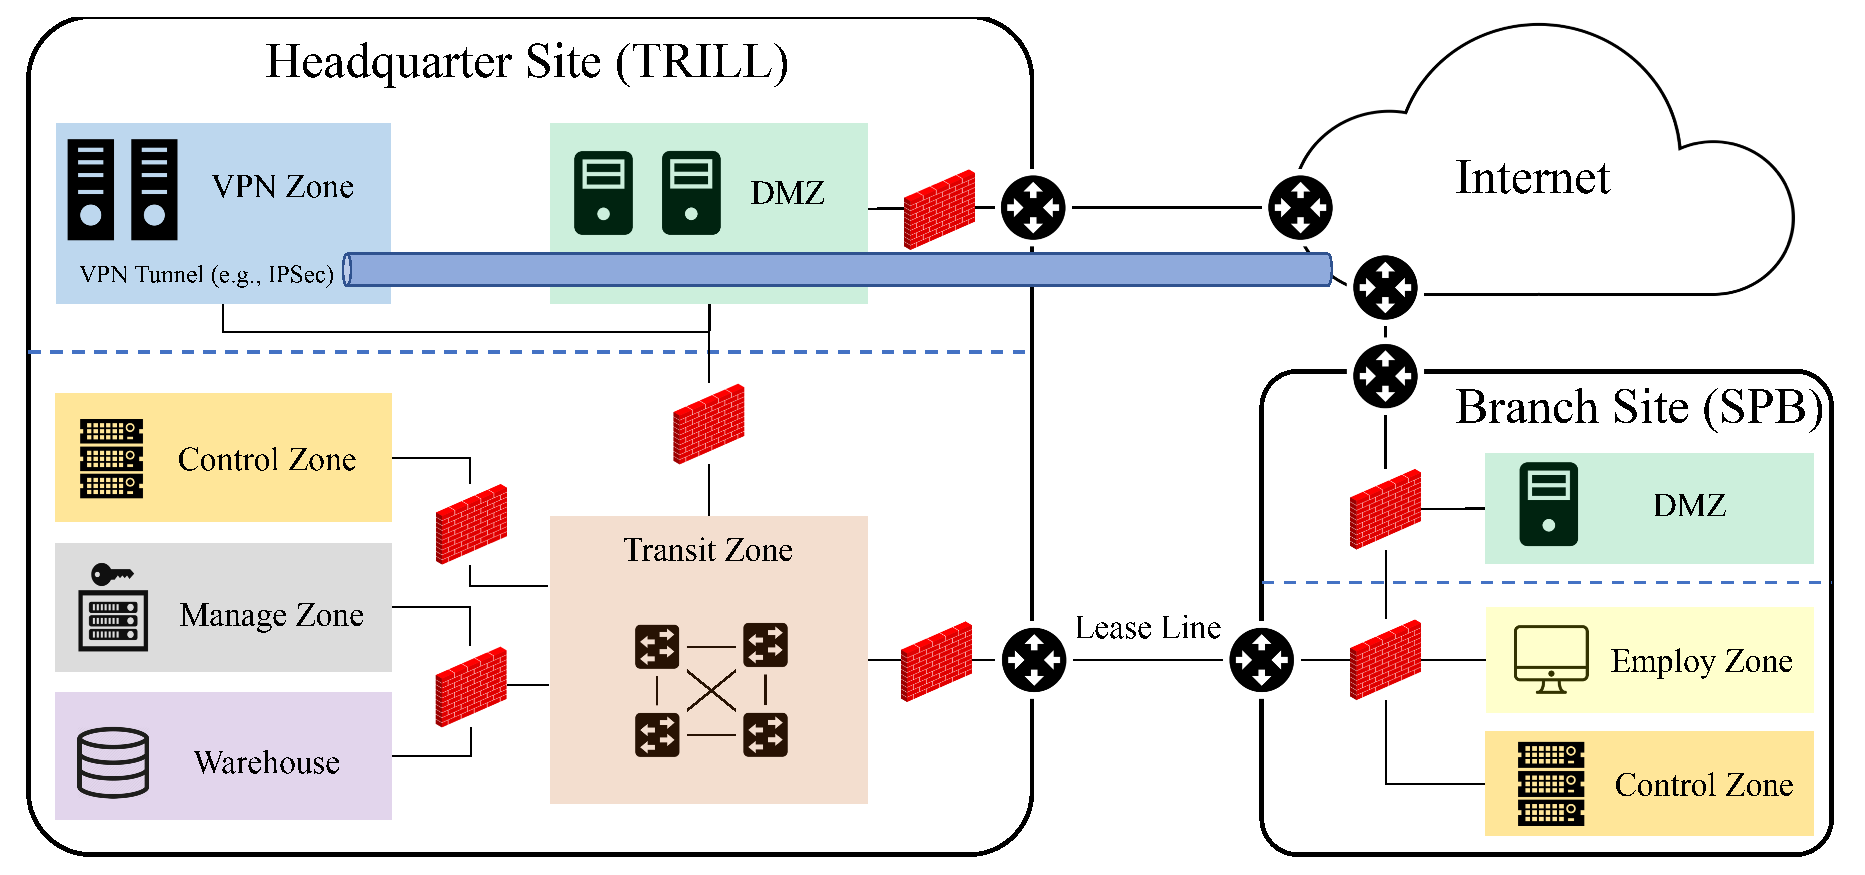
\includegraphics[width=.9\textwidth]{usecase.eps}
	\end{center}
	\caption{\textit{Network zoning use case for large enterprises. Network zones are
	realized with heavy use of security middleboxes (e.g., Firewalls).}}
	\label{fig:usecase}
\end{figure}

Most enterprise networks have embraced the notion of layered security classification,
that can be broadly split into intranet, extranet, and opennet~\cite{ramasamy2011towards}.
The opennet is the least trusted network (e.g., the Internet) which is an inhospitable region
where live threats exist, whereas the intranet is the most trusted network hosting
business-critical systems and sensitive information. Since the intranet has rigorous access
control mechanisms to protect information assets from exposure to the opennet, enterprises are
forced to operate another security layer (extranet, also known as demilitarized zone or DMZ) in between,
which exposes the publicly accessible services to the opennet, while reducing the attack surface of the intranet.

Over time, these layered network structures have become more sophisticated~\cite{obregon2015infrastructure}
due to extreme changes in network environments---diverse demands from customers, partners
and employees accessing enterprise networks with a variety of devices.
As a result, many enterprise networks
comprise a large number of zones defined by operational, organizational, and most
importantly security factors. Figure~\ref{fig:usecase} depicts a real-world use case for
network zones running on inter-domain level with multiple involved autonomous systems (ASes). They
can be categorized into three main types.

\paragraph{Intra-domain Zone Transfer}
% 1. direct transfer
% 2. through trasit zone
Within a local network, multiple devices such as servers, databases, and hosts are connected
through network switches. These devices are assigned with a unique IP address that belongs
to a logically isolated network zone. These zones commonly consist of multiple subnets,
often realized with a layer 2 virtualization technology (e.g., VLAN). Each zone is protected
by a set of security middleboxes, e.g., firewalls, intrusion-prevention systems (IPS),
and intrusion-detection systems (IDS), which enforce predefined security policies for all
traffic passing through.

To maintain the zone-based trust model, access permission to one zone is not considered to be
valid for other zones. That is, an entity must obtain access permissions from all zones on the
path when accessing a non-adjacent zone. This trust model however often complicates policy management
and enforcement, especially for large enterprise networks.
To resolve this complication, the current practice introduces the notion of a dedicated zone in which zone
transitions are handled, called Transit Zone.

\begin{figure}[htb]
	\begin{center}
		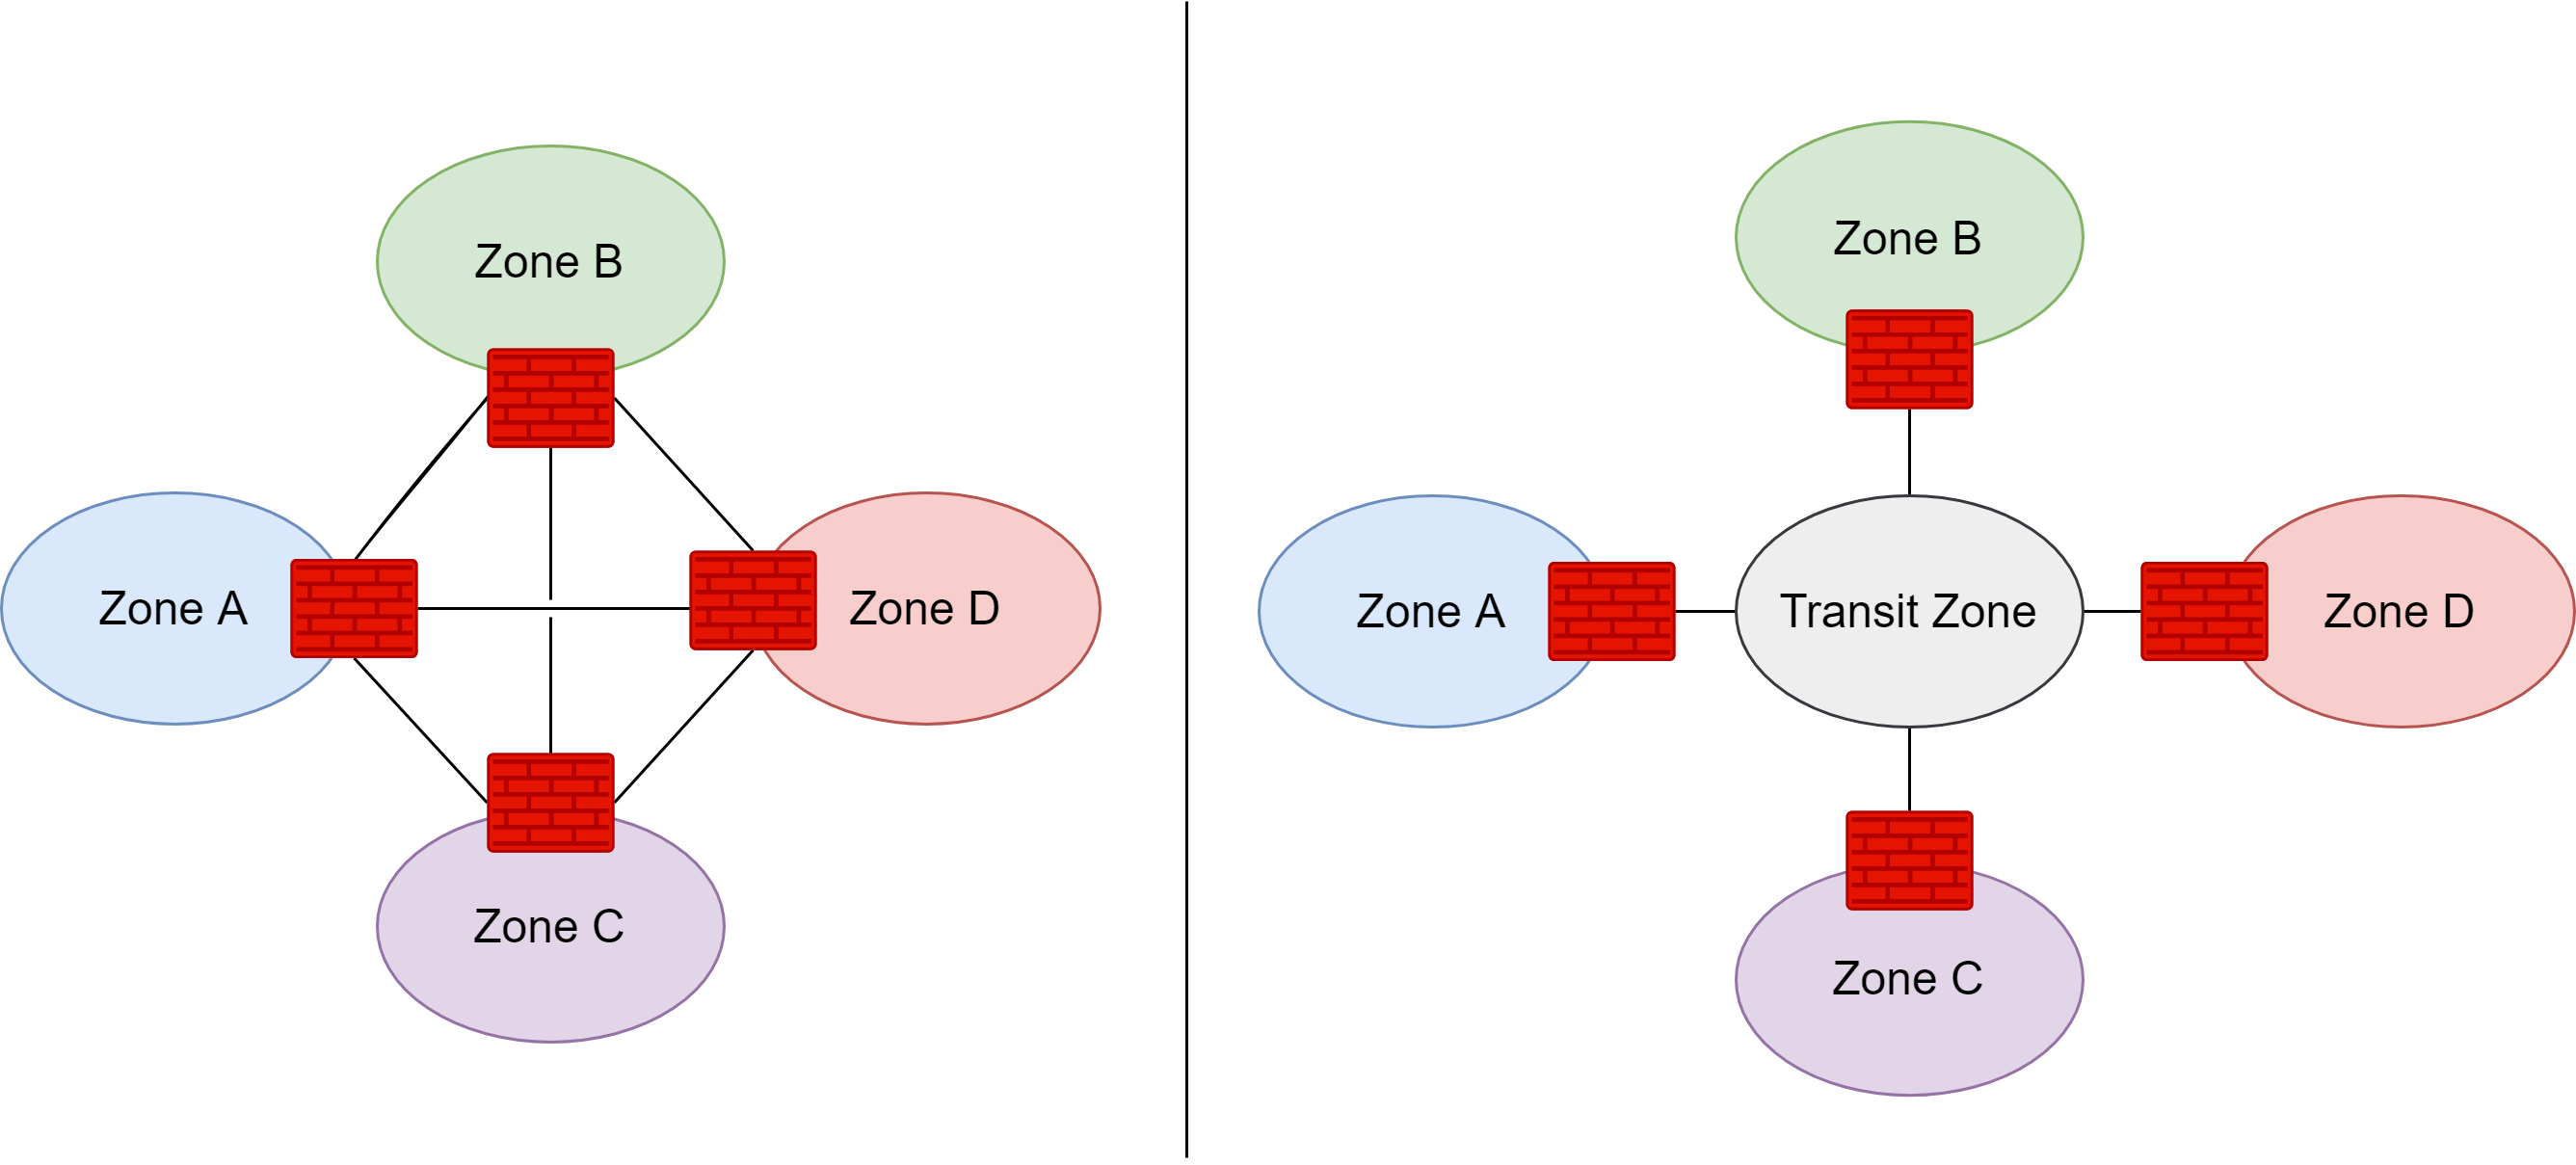
\includegraphics[width=.9\textwidth]{zone_layouts.png}
	\end{center}
	\caption{\textit{Two ways of structuring network zones. The use of a transit zone on the right side reduces
	the number of required links.}}
	\label{fig:zone_layout}
\end{figure}

A transit zone acts like a patch panel allowing zones to be interconnected without the need
of a dedicated link between each pair of zones (Figure~\ref{fig:zone_layout}).
The Transit zone sits in the middle of all
the other zones and mediates access between zones wishing to communicate with each other.
It is commonly comprised of only forwarding devices (e.g., switches), interconnecting the
attached zones via various ingress/egress points on which security middleboxes enforce the
security policies. In a nutshell, the Transit Zone reduces the depth of zone hierarchies and
thus simplifies the network zone design and management.

\paragraph{Inter-domain Zone Transfer}
% briding sites is expensive
To ensure that geographically distributed zones can securely communicate with each other,
enterprises employ various networking technologies. The most common choice is connecting
two remote sites with a physical private line, (e.g., layer 2 circuit). Enterprises
can lease these lines from Internet service providers and make use of them to bridge local
networks. However, purchasing private lines is costly and might come along
with trust issues towards the service provider.

An alternative is a virtual private
network (VPN). A VPN uses cryptographic primitives to create a virtual tunnel between two
local networks, preventing information leakage during transmission over the public Internet.
While the VPN technology ensures data confidentiality, typically yet another layer of overlay
protocols is required to achieve virtual separation of zones. The use of such overlay
protocols, however, has the disadvantage that all interconnected sites need to deploy the same
protocol since such protocols generally do not offer interoperability.

\paragraph{Traffic from the Internet}
% 1. normal customer
% 2. authorised user (employee)
% 3. attacker
Traffic not originating in cooperative (trusted) networks can be classified
into the following three types: i) public traffic, ii) authorized traffic, and iii)
malicious traffic. The first case covers normal customers who access the enterprise's
public services, e.g., Web servers. This traffic in general ends up at the demilitarized zone
(DMZ) hosting only public services that require exposure to Internet.
The second case refers to the traffic coming from temporarily authorized devices. For example,
a legitimate employee outside the enterprise's premises---working from home with a personal
device---may get a temporal permit to access restricted zones via VPN. The last
category comprises attack traffic which is to be filtered by the security middleboxes in the
frontline of defense.

% \begin{table}[t]
% % \caption{use case table. need to be merged with the fig_usecase}
% \label{tab:usecase}
% \centering
% \resizebox{0.48\textwidth}{!}{
% 	\begin{tabular}{*4{c}}
% 	\toprule
% 	& Between Zones & Through Transit Zone & Within Zone\\
% 	\midrule
% 	Inter-domain & \circled{1} $E_1 \leftrightarrow E_4$ 
% 	& \circled{2} $E_1 \leftrightarrow E_5$ & \circled{3} $E_1 \leftrightarrow E_2$\\
% 	Intra-domain & \circled{4} $E_5 \leftrightarrow E_6$ 
% 	& \circled{5} $E_3 \leftrightarrow E_4$ & \circled{6} $E_1 \leftrightarrow E_3$\\
% 	\bottomrule
% 	\end{tabular}
% }
% \end{table}

% \paragraph{Inter-domain Zone Transfer} % Case 1:
% \paragraph{Inter-domain Zone Transfer via Transit} % Case 2: 
% \paragraph{Inter-domain Communication within a Zone} % Case 3: 
% \paragraph{Local Zone Transfer} % Case 4: 
% \paragraph{Local Zone Transfer via Transit} % Case 5: 
% \paragraph{Local Communication within a Zone} % Case 6:
\cmnt{describe all 6 usecases here?}


\section{Challenges}
\label{sec:challenges}

\paragraph{Secure Zone Transfer}
Transmitting security-sensitive data between zones in different physical locations (e.g.,
data center to branch site) over the public Internet poses a challenge.
Security level information is lost in transit, requiring that the data is re-authenticated and
filtered again on the receiving site even though source and destination could be part of the
same logical zone.
Today's overlay protocols are often used to overcome the restriction of losing
security level information in transit. This, however, introduces new challenges: difficulties
in deployment per zone, computational overhead, and poor management scalability.

\paragraph{Interoperability}
Even if security-level information persists in transit, different zones might not be
built on the same internal protocols (e.g., SPB~\cite{ieee2012spb} vs Trill~\cite{rfc6325})
which makes it difficult for end systems in different zones to be able to seamlessly communicate
with each other.
% A new architecture therefore must be able to understand various network protocols and 
% interpret them into a local language that all target networks can understand. This means 
% that the interpretation should preserve the properties of an original protocol, such as 
% % layer-2 routing decisions. 
% virtual segmentation.
% % A flexible design for the architecture to easily embed new protocols also should be considered.
\cmnt{uncomment text, maybe rephrase}

\paragraph{Management Scalability}
In current local network zoning architectures, administration is being considered a tedious,
time-consuming, and labor-intensive task. For example, simply adding a new zone might
require existing policies to be thoroughly reviewed, updated, and re-distributed
to the local network entities. The management complexity dramatically increases in a
wide-area network (WAN) environment.
% For global orchestration across heterogeneous environments, a new architecture therefore
% must ensure management scalability. That is, network administrators should be able to easily extend 
% network zones in different physical locations and update policies that reflect these network
% changes, and be assured that no security loopholes were introduced.
\cmnt{uncomment text, maybe rephrase}

% easily scale up resources 





% \subsection{Industrial Perspectives}

% % \paragraph{Large Enterprise Networks}
% % In order to protect information technology assets, large enterprise networks are partitioned into disjoint segments which group together assets with the same security requirements and policies. These groups are referred to as zones. Zones define the network boundaries and their defense requirements by stating the entities populating the zones, the entry points into the zone as well as how traffic is monitored and filtered at these entry points. Oftentimes, these zones are realized by a (virtualized) separation at layer 2 with firewalls at higher levels governing data transfers between zones.
% Traditionally, enterprises used to consider three security layers for their network 
% environment: intranet, extranet and opennet~\cite{ramasamy2011towards}. The opennet is
% the least trusted network (e.g., the Internet) which is inhospitable region where live 
% threats exist, while the intranet is the most trusted network hosting business-critical 
% systems and sensitive information. Since the intranet has rigorous access controls to 
% protect the information assets from an exposure, enterprises put another security layer 
% (extranet) in between, that only exposes public services to opennet and thus reduces 
% attack surfaces. 
% As enterprises have recently witnessed extreme changes in network environment such as
% diverse demands from customers, partners and employees accessing their network with
% variety of devices, the enterprises employ more sophisticated network security 
% segmentation\cite{obregon2015infrastructure}, called security zones.
% Security zones constitute the logical grouping of one or more subnets that share the
% same security requirements and policies. 
% % Since security zoning is the foundation of 
% % network isolation criteria that must be upheld for secure business environements, 
% % the zone classification of information assets requires 

% Each security zone is identified with different level of trust, and every pair of zones 
% are defined with a namely trusted-untrusted relationship. 
% To realize the unidirectional trust model, firewalls are considered as the most viable
% technologies and widely used in the current practice. However, operating firewalls in 
% large enterprises is often challenging to network operators and security architects. The 
% access control for the security zones might be dynamic, and thus its requires a complex 
% management scheme to accommodate a myriad set of policies. While there are advanced 
% technologies such as virtual firewall~\cite{deng2015vnguard,bakker2016network} and Unified
% Threat Management (UTM)~\cite{qi2007towards}, that are newly designed for enforcement of 
% access control polices in extremely dynamic networks, security zone management and modeling 
% still remains to be evolved~\cite{ramasamy2011towards,gontarczyk2015blueprint}.

% Bridging geographically distant security zones can also be challenging. Oftentimes,
% security zones are created not only for security purpose but also because of geographical
% factors. Given that the security zones in distance should exchange information over
% public network (opennet as aforementioned), there might be a potential risk that the
% communication may expose security-sensitive information during transit. To mitigate
% such a threat, network operators leverage additional security control/mechanisms (e.g.,
% IPSec~\cite{rfc4301} and SSL VPN~\cite{sun2011advantages}) which ensure confidentiality
% and integrity of the transmission over the untrusted network by encrypting the data with
% securely shared cryptographic keys. Nonetheless, the technologies might bring new challenges
% such as management scalability~\cite{felsch2018dangers} and compatibility to the secure 
% isolation~\cite{liu2008collaborative}.

% % \paragraph{Cloud Computing (LaaS, PaaS, SaaS)}
% The cloud computing environment is a good representative example that depicts such practical 
% challenges. Cloud-based service providers operate large multi-tenant data centers which 
% have to scale to customers needs. To achieve this scalability while at the same time staying
% cost efficient cloud providers make heavy use of virtualization techniques. This environment 
% challenges operators with providing secure segmentation between tenants as multiple tenants 
% are using the same physical machines and network. In addition, given that the cloud 
% environments comprise geographically distributed data centers, providing secure communication 
% channels between security zones while upholding a constant view of the security policies
% under the dynamic zone migration is another hill to climb. Now, we derive main challenges 
% we confront in this research with case study.
% % Legal requirements need to be respected. Furthermore, an optimal solution needs to be highly 
% % flexible as the number of assigned resources for a given customer can change frequently.



% % \paragraph{Edge Computing}
% % With the rise of mobile devices and Internet of Things (IoT) new types of data intensive, time
% sensitive applications are emerging. (e.g. VR/AR) However, since these devices are also required to
% be low power they cannot do these heavy computations themselves. Cloud computing can be used to
% offload the work to centralized data centers. However, this causes new challenges. Often, the latency
% between devices and the cloud is too high and therefore not well suited for real-time applications.
% Additionally, a large number of devices means that a centralized infrastructure can get saturated by
% big traffic flows. One widely used solution to this problem is Edge Computing which puts nodes handling
% the computation close to end devices.
 % Background Theory
\chapter{Diagnosing Overthinking}
\label{overthinking}

This chapter presents our framework for identifying and analyzing overthinking behavior in Large Reasoning Models (LRMs). We begin by defining the Reasoning-Action Dilemma that leads to overthinking, then describe the manifestations of this behavior, and finally present our methodology for quantifying it. Through our analysis of 3,908 trajectories, we demonstrate that overthinking represents a significant challenge in agentic environments, particularly affecting models specifically trained for reasoning tasks.

\section{The Reasoning-Action Dilemma}
\label{sec:dilemma_detailed}

We observe that, in agentic decision-making tasks, LRMs constantly face the \emph{Reasoning–Action Dilemma} where they must navigate a fundamental trade-off between:
\begin{itemize}
    \item \textbf{Direct interaction with the environment}, where the model executes actions and receives feedback
    \item \textbf{Internal reasoning}, where the model reasons over hypothetical outcomes before committing to an action
\end{itemize}

Ideally, an LRM should balance reasoning and action by using internal simulation to refine its choices while leveraging real-world feedback to correct errors. For instance, when debugging a failing test case, a well-balanced model would hypothesize potential issues yet still execute the test opportunely to collect concrete failure signals. This balance is particularly critical in software engineering tasks, where models must understand complex codebases, reason about potential fixes, and validate their solutions through testing.

Unfortunately, achieving this balance is inherently challenging. In such settings, feedback is sparse, compelling LRMs to rely heavily on internal simulation to make the most out of every iteration. However, prior research has demonstrated that LRMs exhibit significant vulnerability to knowledge insufficiency, where gaps in understanding can cascade into compounding errors throughout the reasoning process \cite{li2025searcho1agenticsearchenhancedlarge, zhong2024evaluationopenaio1opportunities, LingFLHLMS23, chia2024reasoningpathsoptimizationlearning}. This challenge is exacerbated by LRMs' sensitivity to prompt modifications \cite{openai_learning_to_reason_2024, deepseekai2025deepseekr1incentivizingreasoningcapability}, which can disrupt their ability to maintain and process contextual information. These limitations become especially critical in agentic scenarios, where models must simultaneously gather, retain, and act upon new information \cite{zhang2024agenticinformationretrieval, yang2024sweagentagentcomputerinterfacesenable}. Consequently, excessive simulation without sufficient external information can ultimately lead to failure. The situation is especially difficult for environments with limited interaction opportunities.

\section{Manifestations of Overthinking}
\label{sec:manifestations_detailed}

Our investigation into impaired decision-making in AI agents draws from a detailed analysis of agent-environment interactions. These interactions are recorded in what we term trajectories - comprehensive logs that capture the complete sequence of agent actions, environment responses, and (where available) the agent's reasoning process. As outlined in \cref{evaluation_framework}, we systematically analyzed these trajectories to understand patterns of \textbf{overthinking}.

While most trajectories include the agent's explicit reasoning process, those from the o1 family exclude these reasoning tokens \cite{openai_learning_to_reason_2024}. This limitation led us to focus our analysis on observable behaviors, which are the concrete actions agents take in response to environmental challenges.

Through this analysis, we identified three distinct patterns of \textbf{overthinking}, as illustrated in \cref{fig:manifestations}:

\subsection{Analysis Paralysis}
When faced with challenges, LRMs tend to shift their focus from immediate actions to elaborate future planning. They generate increasingly complex action sequences but struggle to execute them systematically. Rather than addressing immediate errors, they construct intricate plans that often remain unexecuted, leading to a cycle of planning without progress. This behavior is particularly evident in software engineering tasks, where models may spend excessive time analyzing potential code changes without actually implementing and testing them.

\subsection{Rogue Actions}
We observe cases where agents deliberately try to bypass environmental exploration by generating chains of interdependent actions in a single step. Despite their prior demonstrated awareness of step-by-step interaction requirements, models proceed to construct elaborate action sequences that presume the success of each preceding step, effectively substituting real environmental feedback with internal simulation. This behavior often manifests as attempts to execute multiple file modifications or system commands simultaneously, without waiting for confirmation of each step's success.

\subsection{Premature Disengagement}
LRMs sometimes terminate tasks based solely on their internal simulation of the problem space, either through direct abandonment or by delegating hypothetical action sequences. This illustrates how overreliance on internal reasoning can lead to decisions without environmental validation. For example, a model might declare a bug fixed based on its analysis of the code changes, without actually running the tests to verify the fix works as intended.

\section{Quantifying Overthinking}
\label{sec:quantifying}

\subsection{Overthinking Score}
To quantify overthinking behavior, we developed a systematic scoring method using an LLM-based evaluator. This evaluator analyzes model trajectories for the previously described patterns and assigns a score from 0 to 10, with higher scores indicating more severe overthinking behavior. Each score includes a detailed justification explaining which patterns were identified and their severity. The complete evaluation prompt and scoring criteria can be found in \cref{apx:prompt_overthinking}.

Our analysis reveals two distinct patterns in overthinking behavior. First, regression analysis demonstrates a significant negative correlation between overthinking and issue resolution rates for both reasoning and non-reasoning models (\cref{fig:figure1}), with the latter showing a steeper decline in performance as overthinking increases. Second, a direct comparison reveals that reasoning models consistently exhibit higher overthinking scores—nearly three times higher than non-reasoning models—with this difference being statistically significant as shown in \cref{tab:overthinking_scores}.

\subsection{Validation Methodology}
To validate our LLM-based evaluator, we conducted an independent assessment where four expert annotators manually scored 20 randomly selected model traces. The Spearman rank correlation ($p = 0.800$) between human experts and our automated scoring system demonstrated a strong monotonic relationship, as shown in \cref{fig:human_eval}. This non-parametric correlation measure confirms the reliability of our overthinking measurement methodology.

\subsection{Impact on Model Performance}
Statistical analysis reveals that higher overthinking scores correlate with decreased performance across all models. This correlation is particularly strong for reasoning models, which exhibit consistently higher overthinking tendencies, suggesting that excessive reliance on internal simulation impairs task performance. As illustrated in \cref{fig:figure1}, model nomenclature such as "FC" (indicating native function calling capability), "DS" (representing DeepSeek models), and suffixes o1\_high and o1\_low denoting models with reasoning effort set to high and low respectively, all show this consistent pattern.

\subsection{Practical Implications}
Our findings demonstrate that simple efforts to mitigate overthinking can yield substantial benefits. By generating two candidate solutions using o1 with low reasoning effort and selecting the one with lower overthinking score, we not only improved issue resolution from 21\% to 26.3\% on SWE Bench Verified tasks (\cref{fig:figure2}), but also nearly matched the performance of high-reasoning configurations while \textbf{reducing computational costs by approximately 43\%}. This demonstrates that simple overthinking mitigation strategies can dramatically improve the efficiency of LRMs in real-world applications.

\section{Evaluation Framework}
\label{sec:eval_framework}

Our evaluation framework consists of several key components designed to systematically analyze overthinking behavior in LRMs. We employ SWE Bench Verified \cite{jimenez2024swebenchlanguagemodelsresolve, swebench_verified} as our benchmark, using the CodeAct agent scaffolding \cite{wang2024executablecodeactionselicit} within the OpenHands framework \cite{wang2024openhandsopenplatformai}. This setup creates a controlled environment where models must balance information gathering with reasoning chains while maintaining context across multiple interactions as illustrated in \autoref{fig:figure3}.

\subsection{Models Evaluated}
To comprehensively study the phenomenon and influence of overthinking, we consider 19 models across multiple dimensions:
\begin{itemize}
    \item \textbf{Reasoning Capabilities}: Both reasoning-optimized models and general-purpose language models
    \item \textbf{Model Openness}: Proprietary models (e.g., OpenAI o1, Claude Sonnet 3.5) and open-source alternatives (e.g., DeepSeek-R1, Qwen2.5)
    \item \textbf{Model Size}: From small (1.5B-14B) to large-scale models (32B-671B parameters)
    \item \textbf{Function Calling Support}: Models with native function calling capabilities (e.g., OpenAI o1, GPT-4o) versus those without
\end{itemize}

\subsection{Trajectory Analysis}
We analyze complete interaction logs that capture:
\begin{itemize}
    \item Model actions and their timing
    \item Environmental responses
    \item Model's internal reasoning (where available)
    \item Success or failure of task completion
\end{itemize}

Through our analysis of \textbf{3,908 trajectories}, we create a comprehensive open-source dataset to advance research in balancing reasoning and action in agentic environments. Each trajectory is accompanied by its overthinking score and detailed justification.

\subsection{Pattern Recognition}
Our framework systematically identifies instances of:
\begin{itemize}
    \item Extended reasoning chains without action
    \item Multiple action generation in single turns
    \item Premature task termination
    \item Disregard for environmental feedback
\end{itemize}

These patterns are evaluated in the context of software engineering tasks, where we can objectively measure task completion through automated test suites and code validation.

\subsection{Statistical Validation}
Our statistical analysis reveals three key findings about overthinking in language models: its relationship with performance in SWE-bench, its non-equal prevalence across model types, and its practical implications for model selection. We employ rigorous statistical methods to ensure the reliability of our findings.

Regression analysis demonstrates a significant negative correlation between overthinking and issue resolution rates for both reasoning and non-reasoning models. Non-reasoning models show a steeper decline in performance as overthinking increases, with a beta coefficient of -25.802 compared to -11.476 for reasoning models. Both relationships are statistically significant (p = 0.031 and p = 0.006 respectively).

A direct comparison reveals that reasoning models consistently exhibit higher overthinking scores—nearly three times higher than non-reasoning models. Reasoning models average 2.320 ± 1.120 on our overthinking scale, while non-reasoning models score 0.865 ± 0.432. This difference is statistically significant (p = 0.019), suggesting a systematic tendency toward overthinking in reasoning-optimized models.

To validate our automated scoring system, we conducted an independent assessment with four expert annotators who manually scored 20 randomly selected model traces. The Spearman rank correlation (p = 0.800) between human experts and our automated system demonstrates a strong monotonic relationship, confirming the reliability of our measurement methodology.

The complete analytical framework and results are presented in \cref{evaluation_framework}. The tools used for the statistical analysis can be found in \cref{stat_framework}.

\section{Implementation Details}
\label{sec:implementation}

\subsection{LLM-as-Judge System}
Following the LLM-as-a-judge methodology \cite{zheng2023judgingllmasajudgemtbenchchatbot}, our evaluation system uses Claude Sonnet 3.5 as the judge model, configured with:
\begin{itemize}
    \item Temperature set to 0 for deterministic scoring
    \item 200k token context window to process full trajectories
    \item Structured output format for consistent scoring
    \item Detailed justification requirements for transparency
\end{itemize}

Claude Sonnet 3.5 was selected for its extensive context window, allowing it to process complete trajectories alongside the evaluation criteria. Notably, the evaluator does not have access to the final issue resolution outcome, ensuring that the overthinking assessment remains independent of task success and thereby eliminating potential biases.

\subsection{Scoring Criteria}
The scoring system evaluates trajectories on multiple dimensions:
\begin{itemize}
    \item Balance between reasoning and action
    \item Appropriate use of environmental feedback
    \item Efficiency of problem-solving approach
    \item Completion of necessary validation steps
\end{itemize}

\subsection{Model Size and Overthinking}
Our initial hypothesis posited that smaller LRMs would struggle more with environmental comprehension, leading them to rely heavily on internal reasoning chains and thus exhibit increased overthinking behavior. To test this hypothesis, we analyzed two model families across four size variants (32B, 14B, 7B, and 1.5B): the non-reasoning Qwen2.5-Instruct and the reasoning R1-Distill-Qwen.

Our analysis revealed a strong negative correlation between model size and overthinking scores: larger models demonstrated less tendency to overthink, as shown in \cref{figure5}. The distinction between reasoning and non-reasoning models becomes particularly pronounced at smaller scales. R1 models exhibit significantly higher overthinking scores (5.157 ± 2.292) compared to their Qwen2.5 counterparts (1.771 ± 0.463), with this gap widening as model size decreases. This difference is statistically significant (t = 2.508, p = 0.046).

\subsection{Token Usage Analysis}
We investigated the relationship between token consumption and overthinking behavior in the o1 model. We conducted experiments by manipulating the model's reasoning effort parameter between high and low settings, which influences the number of reasoning tokens used \cite{openai_chat_api}. Our analysis revealed an unexpected pattern: in agent-based scenarios, o1 models with low reasoning effort demonstrated 35\% higher overthinking scores compared to their high-effort counterparts. As shown in \cref{tab:o1_model_comparison}, the difference in averaged overthinking scores between the two configurations is statistically significant, suggesting that increased token allocation might paradoxically reduce overthinking in agentic contexts.

\subsection{Function Calling Impact}
Our experimental analysis compared O1 model configurations with high reasoning effort, evaluating performance both with and without native function calling (FC) capabilities. The integration of FC capabilities yielded substantial improvements:
\begin{itemize}
    \item Performance score increased from 29.1\% to 47.7\%
    \item Average overthinking score reduced from 2.47 to 0.56
\end{itemize}

However, benchmarking against BCFL \cite{berkeley-function-calling-leaderboard} reveals a more nuanced pattern, where the performance differential between FC and non-FC implementations of O1 in multi-turn environments shows a modest improvement from 36\% to 41\%. This comparatively smaller enhancement suggests that FC implementation alone cannot fully account for the dramatic performance improvements observed in our primary experiments.

OpenAI has demonstrated that reasoning models exhibit a disproportionate increase in computational costs relative to their performance gains \cite{arcprize2024oai}. Our experiments with SWE-bench Verified dataset confirm this observation: o1 with high reasoning effort achieves a 29.1\% resolution rate at \$1,400, while the low reasoning variant reaches 21.0\% at \$400—a 3.5x cost difference for an 8.1 percentage point improvement in performance.

To address this efficiency gap, we developed an alternative approach: running the low-reasoning variant twice and selecting traces with minimal overthinking scores. This method achieved a 26.3\% resolution rate while consuming only 57\% of the high-reasoning configuration's cost. Our findings suggest that monitoring and controlling overthinking behavior could be a cost-effective strategy for optimizing model performance in real-world applications.

\section{Limitations and Considerations}
\label{sec:limitations}

While our framework provides valuable insights into overthinking behavior, it has several limitations that inform our ongoing research directions:

\subsection{Technical Limitations}
\begin{itemize}
    \item \textbf{Limited Access to Internal Reasoning}: Models like o1 exclude reasoning tokens \cite{openai_learning_to_reason_2024}, forcing us to rely on observable behaviors. This limitation may obscure some aspects of the overthinking process.
    
    \item \textbf{Potential Bias in LLM-based Evaluation}: While our LLM-as-judge approach shows strong correlation with human evaluators, the use of Claude Sonnet 3.5 as an evaluator may introduce its own biases in overthinking detection.
    
    \item \textbf{Computational Cost}: Processing and analyzing 3,908 trajectories requires significant computational resources, particularly for models with high reasoning effort settings.
    
    \item \textbf{Scalability Challenges}: The current framework may face challenges scaling to larger datasets or more complex interaction patterns.
\end{itemize}

\subsection{Methodological Considerations}
\begin{itemize}
    \item \textbf{Pattern Identification}: While we've identified three main patterns of overthinking, there may be other manifestations that our current framework doesn't capture.
    
    \item \textbf{Human Validation Process}: The complexity of validating overthinking scores requires significant expert time and may not scale well to larger studies.
    
    \item \textbf{Domain Specificity}: Our findings are primarily based on software engineering tasks using SWE Bench Verified. The patterns and implications may differ in other domains.
    
    \item \textbf{Model Size Effects}: Our analysis of DeepSeek-R1-671B revealed overthinking scores comparable to DeepSeek-V3-671B, suggesting that model scale and training methodology interact in complex ways that warrant further investigation.
\end{itemize}

\subsection{Future Research Directions}
Our analysis suggests two promising approaches to mitigate overthinking in LRMs:

\begin{itemize}
    \item \textbf{Native Function-Calling}: The success of function-calling architectures hints at the importance of explicit interaction training, though our BCFL benchmarking suggests this alone isn't sufficient.
    
    \item \textbf{Selective Reinforcement Learning}: The effectiveness of limited reinforcement learning in DeepSeek-R1-671B points to the role of training methodology in controlling overthinking tendencies.
\end{itemize}

These insights open important questions for future research:
\begin{itemize}
    \item How do these approaches generalize across different domains?
    \item How can we optimize for environments where environmental interaction carries varying costs?
    \item What role does model scale play in overthinking behavior?
\end{itemize}

Understanding these dynamics could help develop more robust solutions that prevent, rather than just mitigate, overthinking behaviors in large reasoning models. To facilitate further research in this direction, we release our evaluation framework and dataset of 3,908 trajectories, enabling the broader research community to build upon these findings across different environments and architectures.
 % Diagnosing Overthinking
\chapter{Evaluation}
\label{eval}

% With the prototype implementation, we conduct extensive evaluation including 
% system/network-wide benchmarks. 

\section{System Benchmarks}
\label{sec:systembenchmark}

% \paragraph{Experimental Setup}
We first conduct microbenchmark tests to evaluate the performance of \tp including the key
derivation, packet authentication, and authorization. For scrutinize and reproducible evaluation,
we leverage the standard benchmark library \texttt{testing} officially supported by golang.
The benchmarks are conducted on commodity machines equipped with an Intel i7 \SI{2.9}{GHz}
CPU, \SI{16}{GB} memory, and a \SI{1}{GbE} NIC.

\begin{table}[htb]
	\begin{minipage}{.47\linewidth}
		\caption{Benchmark results for the transfer policy lookup (ns).}
		\label{tab:authorization}
		\begin{tabularx}{1\linewidth}{X|XXXX}
			\toprule
			\# of Policies & No Miss & Src IP Miss & Dest IP Miss & Policy Miss \\
			\midrule
			100            & 312     & 100         & 235          & 313         \\
			\SI{1}{K}      & 399     & 105         & 264          & 394         \\
			\SI{10}{K}     & 381     & 99          & 262          & 386         \\
			\SI{100}{K}    & 448     & 101         & 290          & 435         \\
			\bottomrule
		\end{tabularx}
	\end{minipage}\hspace{2em}
	\begin{minipage}{.47\linewidth}
		\caption{Sender-side L1 key lookup and L2 key derivation times for different network sizes (ns).}
		\label{tab:derivation_send}
		\begin{tabularx}{1\linewidth}{X|XX}
			\toprule
			\# of Branches & 1st-level Key & 2nd-level Key \\
			\midrule
			100            & 154           & 88            \\	% 618-530=88
			\SI{1}{K}      & 155           & 97            \\	% 627-530=97
			\SI{10}{K}     & 161           & 175           \\	% 705-530=175
			\SI{100}{K}    & 157           & 111           \\	% 641-530=111
			\bottomrule
		\end{tabularx}
	\end{minipage}\vspace{2em}
	\begin{minipage}{.47\linewidth}
		\caption{Receiver-side L1/L2 key derivation times for different network sizes (ns).}
		\label{tab:derivation_rec}
		\begin{tabularx}{1\linewidth}{X|XX}
			\toprule
			\# of Branches & 1st-level Key & 2nd-level Key \\
			\midrule
			100            & 188           & 104           \\	% 508-404=104
			\SI{1}{K}      & 188           & 104           \\	% 508-404=104
			\SI{10}{K}     & 197           & 103           \\	% 507-404=103
			\SI{100}{K}    & 188           & 104           \\	% 508-404=104
			\bottomrule
		\end{tabularx}
	\end{minipage}\hspace{2em}
	\begin{minipage}{.47\linewidth}
		\caption{Processing times for the encryption/decryption for different packet sizes (ns).}
		\label{tab:authentication}
		\begin{tabularx}{1\linewidth}{X|XX}
			\toprule
			Packet Size (byte) & Encryption & Decryption \\
			\midrule
			100                & 856        & 659        \\
			500                & 1082       & 747        \\
			1000               & 1338       & 850        \\
			1500               & 1557       & 950        \\
			\bottomrule
		\end{tabularx}
	\end{minipage}
\end{table}

\paragraph{Authorization}
% The \tp's transfer module performs zone transfer authorization for every incoming packets.
\cmnt{adapt text to reflect new table}
From a technical perspective, the zone transfer authorization consists of two tree searches followed
by a database lookup;
upon receiving the packet metadata from the core module, the transfer module first looks
up the corresponding zone identifiers for the source and destination addresses, and then
compares them to the zone transfer policies. The authorization performance is therefore
dependent on the lookup time of the trees and the policy database.

Table~\ref{tab:authorization} shows
the benchmark results of database lookups for different numbers of policies.
Note that each benchmark ran a couple million iterations and kept the mean value.
The authorization check takes approximately 300 to \SI{500}{ns} per packet, which is a
notable result considering: i) a single lookup consists of two tree searches and a database lookup, ii) the result
is from a high-level language implementation, and iii) the test set scales 1000 times.
As expected, a lookup failure is commonly 24 to 31~\% faster than a successful lookup.
This implies that abnormal packets with invalid zone transfer requests can be quickly
discarded.


\paragraph{Key Derivation}
% When a \tp handles an inter-domain zone transfer packet, the \tp need to derive a correct 
% key for the authentication. As we described in~\S\ref{ssec:keymanagement}, the key derivation
% comprise with two steps: fetch the first-level key from the cache, and dynamically derive the 
% second-level key from the first-level key. 
% To securely forward a zone transfer packet over the public Internet, a \tp first 
We investigate the key derivation performance. Recall that the key derivation proceeds
differently for sender and receiver. A receiver is capable of directly deriving the
second-level key from the local secret (Eq.~\ref{eq:1stkey} \& Eq.~\ref{eq:2ndkey}),
whereas a sender needs to fetch the first-level key from the key cache before it can derive the second-level key.
From a scalability perspective, we vary the number of branches (a \tp for each) by increasing the number of stored
first-level keys up to \SI{100}{K}. Table~\ref{tab:derivation_send} depicts the average time for sender-side key derivation
measured by a benchmark running more than a million iterations. Table~\ref{tab:derivation_rec} shows the same results for
receiver-side key derivation. As can be seen, looking up the first-level key from cache is slightly faster than
deriving the first-level key from the local secret. This is expected when using a high-level language like golang.
Much faster key derivations are possible when using a state-of-the-art implementation \cite{rot2020piskes}.
On the other hand, the second-level key derivation takes roughly the same amount of time for sender- and receiver-side.
This is to be exptected as this derivation step is identical in both cases.

We observe that the lookup time for the first-level key is independent of the size of the key
table, taking between \SI{154}{ns} and \SI{161}{ns}. In addition, the size of the key table is
also irrelevant for the second-level key derivation
because second-level keys are directly derived from first-level keys.
The results indicate that the processing time for a key derivation is less than 1 $\mu$s
even in very large networks with \SI{100}{K} branch sites, which is negligible considering
network latency in today's Internet.

\paragraph{Authentication}
The additional processing time for packet encryption and decryption is shown in
Table~\ref{tab:authentication}. In summary, it requires approximately 1.5 to 2.5 $\mu$s to
authenticate various sizes of packets. We note that the processing overhead occurs for the majority
of tunneling technologies that provide confidentiality for data transmission. The processing
time can be minimized with implementations using the Data Plane Development Kit
(DPDK)~\cite{dpdk} or by leveraging hardware dedicated to cryptographic
operations.

\section{Network Benchmarks}
\label{sec:networkbenchmark}

\begin{figure}[htb]
	\begin{minipage}{.47\linewidth}
		\centering
		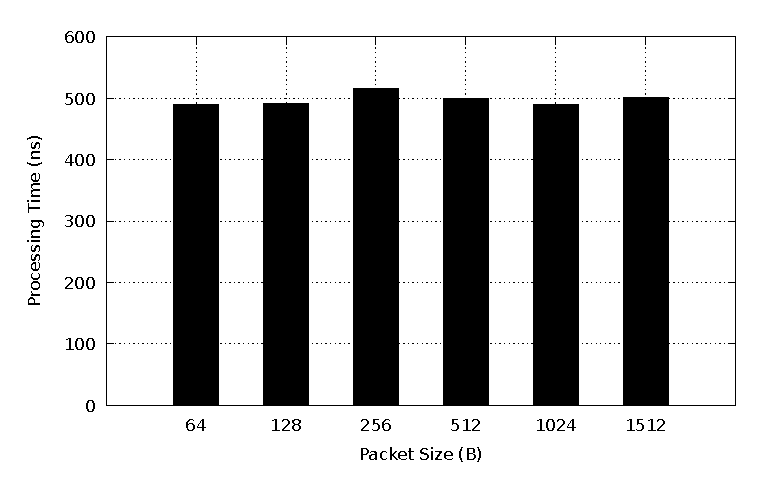
\includegraphics[width=\linewidth]{intra.eps}
		\caption{Processing time for intra-domain zone transfer.}
		\label{fig:intra}
	\end{minipage}\hspace{1em}
	\begin{minipage}{.47\linewidth}
		\centering
		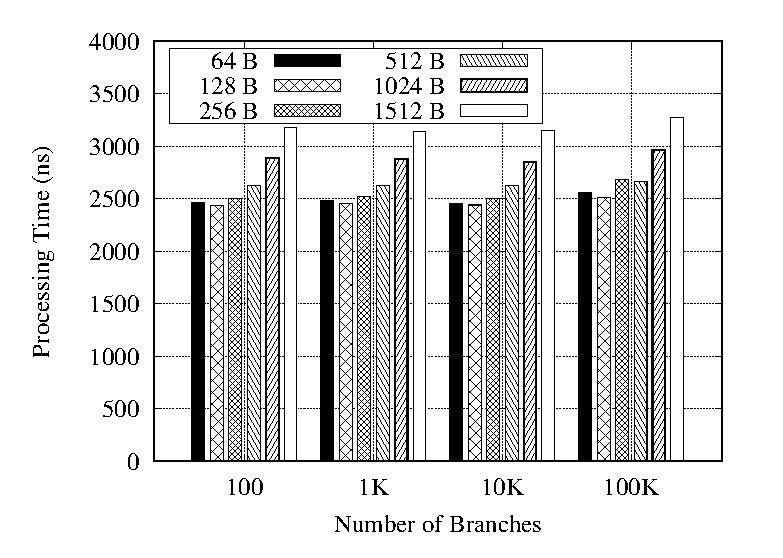
\includegraphics[width=\linewidth]{inter_sender.eps}
		\caption{Processing time on $TP_S$ for inter-domain zone transfer.}
		\label{fig:inter_sender}
	\end{minipage}\vspace{2em}
	\begin{minipage}{.47\linewidth}
		\centering
		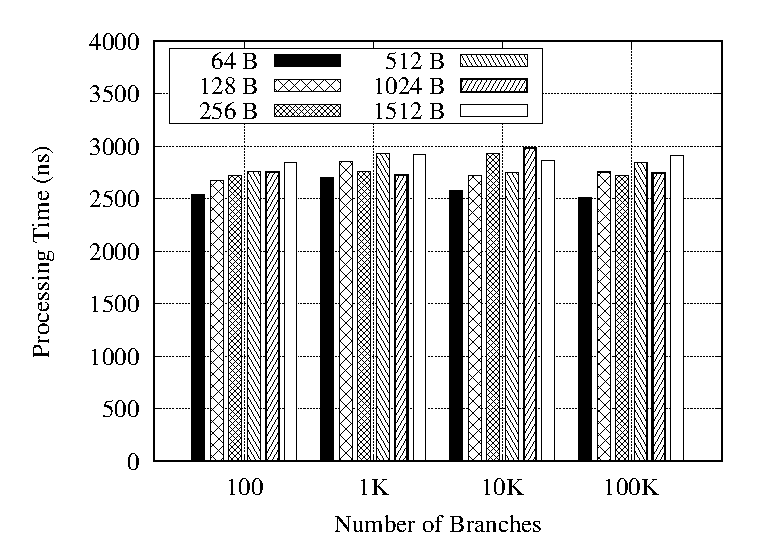
\includegraphics[width=\linewidth]{inter_receiver.eps}
		\caption{Processing time on $TP_R$ for inter-domain zone transfer.}
		\label{fig:inter_receiver}
	\end{minipage}\hspace{1em}
	\begin{minipage}{.47\linewidth}
		\centering
		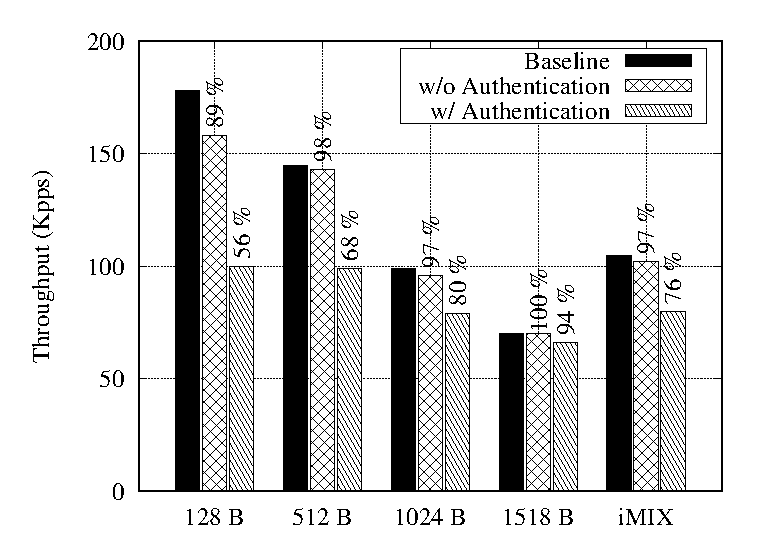
\includegraphics[width=\linewidth]{pps.eps}
		\caption{Forwarding performance of \tp for various size of packets.}
		\label{fig:forwarding}
	\end{minipage}\vspace{2em}
	\begin{minipage}{.47\linewidth}
		\centering
		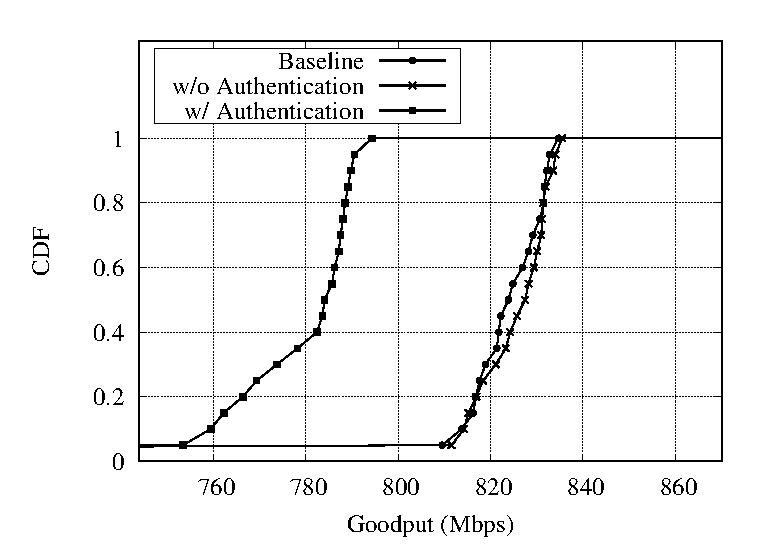
\includegraphics[width=\linewidth]{cdf_goodput.eps}
		\caption{CDF of goodput for 1400-bytes of maximum segment size (MMS).}
		\label{fig:goodput}
	\end{minipage}\hspace{1em}
	\begin{minipage}{.47\linewidth}
		\centering
		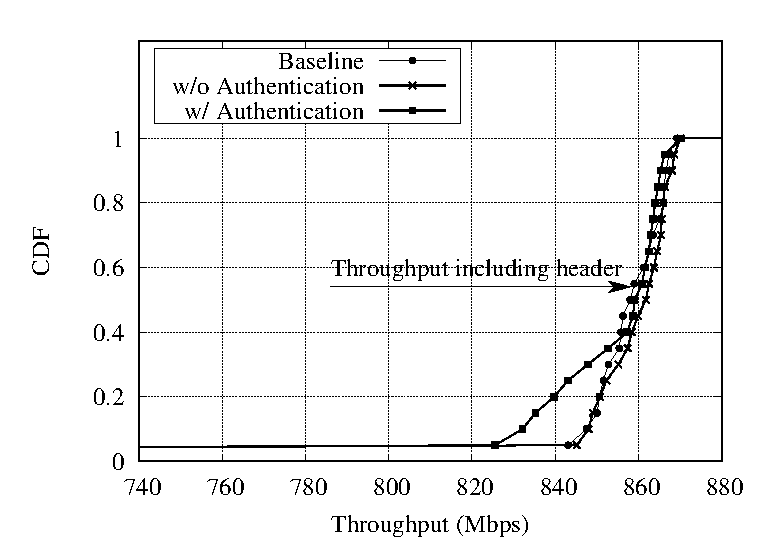
\includegraphics[width=\linewidth]{cdf_throughput.eps}
		\caption{CDF of throughput including extra header fields.}
		\label{fig:throughput}
	\end{minipage}
\end{figure}

So far, we evaluated the performance of each instruction newly introduced. Since a different
set of instructions needs to be applied depending on the zone transfer use case, it is also
important to investigate the overall network performance for handling different types of zone
transfer packets. We now benchmark the actual network performance for both intra- and inter-domain
zone transfer cases.

\paragraph{Latency Inflation}
Figure~\ref{fig:intra} illustrates the network benchmark results for the intra-domain zone
transfer where the source and destination zones are within the same local network, such that
the \tp only performs zone transfer authorization. Since no cryptographic operations are involved,
the additional latency is negligible (as a single legitimate zone transfer takes $\sim$
\SI{500}{ns}). There might be an authorization abort due to a lookup failure that could be
caused by the following three reasons: no matching source zone ID, destination zone ID, or
zone transfer policy. In our prototype, the lookups are performed sequentially and thus
there are different processing overheads (\SI{100}{ns} $\sim$ \SI{450}{ns}) depending on when a
lookup failure occurs. Nevertheless, in case there exists no valid zone-transfer policy, the
packet will be simply dropped and therefore no additional latency is caused.

For inter-domain zone transfer cases, we benchmark the overall network inflation during \tp
operations including packet parsing, key derivation, authorization, and authentication.
Figure~\ref{fig:inter_sender} and~\ref{fig:inter_receiver} depict the processing delay from
sender-side \tp and receiver-side \tp, respectively.
From the results, we make the following observations: first, the overall latency inflation that
\name introduces is insignificant ($\sim 3 \mu$s). Second, \name scales well with the size of the
network, i.e., the number of branches. We do not see any notable performance degradation
($\leq$ \SI{200}{ns}). Third, the size of a packet is the primary factor for the latency increment
as expected for all data-plane devices. The packet size has a small latency incremental factor of
1.28 (i.e, 2.4 $\mu$s to 3.8 $\mu$s). Lastly, we observe no significant bias in network
performance between sender-side and receiver-side \tps.


\paragraph{Forwarding Performance}
We further investigate the actual forwarding performance for various packet sizes (\SI{128}{B},
\SI{256}{B}, \SI{512}{B}, \SI{1024}{B}) including a representative mixture of Internet traffic
(iMIX)~\cite{rfc6985}; we select the minimum packet size of 128 bytes instead of 64 bytes which is
commonly considered to be the smallest packet size, because \name's tunneling requires an at least 116
bytes long frame, i.e., Outer L3 header (40 bytes), AT header
(36 bytes), and EIP (40 bytes). Figure~\ref{fig:forwarding} shows the results. The
baseline is the forwarding performance without \tp operations. The other bars represent the
forwarding performance for intra-domain zone transfer (with authorization only) and inter-domain
zone transfer (with authorization and authentication) respectively.

For 128-byte packets which demonstrates the highest packet rate, and thus requiring the most
extreme packet processing, the intra-domain zone transfer exhibits a throughput degradation
of only 11\%. For other packet sizes we achieve a throughput of 97 $\sim$ 100\%. These
results are expected because \tps only perform zone authorization for intra-domain zone transfer
packets, which increases processing delay by $\leq$ 500 ns. Considering that
a typical intra-domain packet transmission usually shows a few milliseconds of latency, the
additional delay is negligible.

On the other hand, the inter-domain zone transfer degrades the throughput by 44\% for the
smallest packets. Although the degradation diminishes as the packet size increases, the
performance still degrades by 24\% for the iMIX traffic. To investigate the main degradation
factor, we compare the amount of transmitted data (goodput) and the total bits transmitted
including all the network headers (throughputs) as shown in Figure~\ref{fig:goodput} and
\ref{fig:throughput}. From the comparison, we observe the followings: i) the inter-domain
zone transfer achieves a similar throughput to the baseline if the extra headers are considered,
ii) the performance degradation is caused by not only the additional processing delay but also
transmission delay of the extra headers, and therefore iii) \name performs similar to
today's tunneling applications while providing security policy enforcement for network
zoning.



% \subsection{Overhead Measurements}
% \label{ssec:overhead}

% \paragraph{Bandwidth Overhead}

% \paragraph{Memory Overhead}

% \paragraph{Control-plan Overhead}

 % Evaluation
\chapter{Results}
\label{results}

We generate and evaluate \textbf{3908 trajectories} using our evaluation methodology across all models. We make publicly available every trajectory alongside their corresponding overthinking score and the reasoning behind this score.

Our analysis reveals three key findings about overthinking in language models: its relationship with performance in SWE-bench, its non-equal prevalence across model types, and its practical implications for model selection. We observed that overthinking consistently impacts performance across all evaluated models, with reasoning-optimized models showing higher overthinking tendencies than general-purpose ones.

\section{Overthinking and Performance}
\label{sec:perf}

We anticipated that overthinking should impact performance as if models rely too heavily on their internal reasoning chain, there is a high likelihood that they will propose fixes based on inaccurate claims.

We observed a strong negative correlation between overthinking and performance on SWE-bench, as illustrated in \cref{fig:figure1}. Both reasoning and non-reasoning models show decreased performance as overthinking increases, though with notably different patterns.

\section{Overthinking and Model Type}
\label{sec:model_type}

We make three key observations with regards to overthinking in reasoning and non-reasoning models:

\subsection{Non-reasoning Models Can Overthink}
This observation can be explained by the presence of reasoning capabilities in non-reasoning models which could lead to overthinking. Recent studies show that non-reasoning models could have reasoning capabilities \cite{wei2023chainofthoughtpromptingelicitsreasoning, yao2023treethoughtsdeliberateproblem, chen2023program, kojima2023largelanguagemodelszeroshot}.

\subsection{Higher Overthinking in Reasoning Models}
Reasoning models significantly have higher overthinking scores compared to non-reasoning models, as shown in \cref{tab:overthinking_scores}. Since these models are specifically trained to reason and generate extended chains of thought by simulating environment interaction, they are more likely to suffer from manifestations of overthinking.

\subsection{Severe Impact on Non-reasoning Models}
Non-reasoning models that overthink suffer from severe degradation in issue resolution, as evidenced by the beta coefficients shown in \cref{tab:regression_results}. Lower beta coefficients indicate higher impact of overthinking on performance. We suspect that since non-reasoning models are not trained for reasoning, they are not capable of handling reasoning chains effectively, thus showing worse results.

\begin{table}[ht]
\centering
\begin{tabular}{lcccc}
\toprule
\textbf{Model} & \boldmath{$\beta_1$} & \boldmath{$R^2$} & \textbf{p-value} \\
\midrule
Reasoning      & -11.476 & 0.808 & 0.006 \\
Non-Reasoning  & -25.802 & 0.727 & 0.031 \\
\bottomrule
\end{tabular}
\caption{Regression Results for Reasoning and Non-Reasoning Models}
\label{tab:regression_results}
\end{table}

\begin{table}[ht]
\centering
\begin{tabular}{lc}
\toprule
\textbf{Measure} & \textbf{Value} \\
\midrule
Reasoning Models       & 2.320 $\pm$ 1.120 \\
Non-Reasoning Models   & 0.865 $\pm$ 0.432 \\
\midrule
T-test p-value         & 0.019 \\
\bottomrule
\end{tabular}
\caption{Average Overthinking Scores for Reasoning and Non-Reasoning Models}
\label{tab:overthinking_scores}
\end{table}

\section{Overthinking and Model Size}
\label{sec:model_size}

We analyzed two model families across four size variants (32B, 14B, 7B, and 1.5B): the non-reasoning Qwen2.5-Instruct \cite{qwen2,qwen2.5} and the reasoning R1-Distill-Qwen \cite{deepseekai2025deepseekr1incentivizingreasoningcapability}. Our analysis revealed two key patterns:

\begin{enumerate}
    \item Larger models demonstrate less tendency to overthink
    \item The gap in overthinking scores between reasoning and non-reasoning models widens at smaller scales
\end{enumerate}

As detailed in \cref{tab:overthinking_comparison}, R1 models exhibit significantly higher overthinking scores compared to their Qwen2.5 counterparts, with this gap widening as model size decreases.

\begin{table}[ht]
\centering
\begin{tabular}{lccc}
\bottomrule
\textbf{Measure} & \textbf{Value} \\
\midrule
DS-R1 Family        & 5.157 $\pm$ 2.292 \\
Qwen2.5 Family      & 1.771 $\pm$ 0.463 \\
\midrule
T-test statistic     & 2.508 \\
T-test p-value       & 0.046 \\
\bottomrule
\end{tabular}
\caption{Overthinking Score Comparison for R1 and Qwen2.5}
\label{tab:overthinking_comparison}
\end{table}

\section{Overthinking and Token Usage}
\label{sec:token_usage}

We investigated the relationship between token consumption and overthinking behavior in the o1 model by manipulating the model's reasoning effort parameter between high and low settings. Our analysis revealed that o1 models with low reasoning effort demonstrate 35\% higher overthinking scores compared to their high-effort counterparts.

As shown in \cref{tab:o1_model_comparison}, the difference in averaged overthinking scores between the two configurations is statistically significant, suggesting that increased token allocation might reduce overthinking in agentic contexts.

\begin{table}[ht]
\centering
\begin{tabular}{lc}
\toprule
\textbf{Measure} & \textbf{Value} \\
\midrule
O1 Low        & 3.327 $\pm$ 4.539 \\
O1 High       & 2.467 $\pm$ 4.123 \\
\midrule
T-test p-value & 0.050 \\
\bottomrule
\end{tabular}
\caption{Comparison of o1 Models with Different Reasoning Efforts}
\label{tab:o1_model_comparison}
\end{table}

\section{Overthinking and Context Window}
\label{sec:context_window}

When comparing models of similar size but different context windows—such as DS-R1-32B versus QwQ and GPT-4o-mini versus SkyT1—we found no consistent relationship between context window size and overthinking tendencies. These observations suggest that context window size may not be a primary factor in determining a model's propensity for overthinking.

\section{Practical Implications}
\label{sec:implications}

OpenAI has demonstrated that reasoning models exhibit a disproportionate increase in computational costs relative to their performance gains \cite{arcprize2024oai}. Our experiments with SWE-bench Verified dataset confirm this observation: o1 with high reasoning effort achieves a 29.1\% resolution rate at \$1,400, while the low reasoning variant reaches 21.0\% at \$400—a 3.5x cost difference for an 8.1 percentage point improvement in performance.

To address this efficiency gap, we developed an alternative approach: running the low-reasoning variant twice and selecting traces with minimal overthinking scores. This method achieved a \textit{26.3\% resolution rate while consuming only 57\% of the high-reasoning configuration's cost}, as shown in \cref{fig:figure2}. Our findings suggest that monitoring and controlling overthinking behavior could be a cost-effective strategy for optimizing model performance in real-world applications. % Results
\chapter{Discussion}
\label{discussion}

\section{Native Function Calling Impact}
\label{sec:function_calling}

Our experimental analysis compared O1 model configurations with high reasoning effort, evaluating performance both with and without native function calling (FC) capabilities. The integration of FC capabilities yielded substantial improvements, increasing the performance score from 29.1\% to 47.7\%, while simultaneously reducing the average overthinking score from 2.47 to 0.56 -- effectively mitigating the overthinking phenomenon.

However, benchmarking against BCFL \cite{berkeley-function-calling-leaderboard} reveals a more nuanced pattern, where the performance differential between FC and non-FC implementations of O1 in multi-turn environments shows a modest improvement from 36\% to 41\%. This comparatively smaller enhancement suggests that FC implementation alone cannot fully account for the dramatic performance improvements observed in our primary experiments.

\section{The Case of DeepSeek-R1-671B}
\label{sec:deepseek}

Our analysis of DeepSeek-R1-671B (DS-R1) revealed overthinking scores comparable to those of DeepSeek-V3-671B. This similarity in overthinking behavior may be attributed to DS-R1's training methodology, which did not incorporate extensive reinforcement learning for software engineering tasks. While DS-R1 maintains performance levels similar to DeepSeek-V3 on software engineering benchmarks \cite{deepseekai2025deepseekr1incentivizingreasoningcapability}, our findings suggest that the combination of limited RL training and substantial model scale (671B parameters) contributed to its controlled overthinking behavior.

\section{How to Fix Overthinking}
\label{sec:solutions}

While our algorithmic interventions demonstrate immediate practical benefits, they primarily address the symptoms rather than the root causes of overthinking. Our analysis suggests that more fundamental solutions might emerge from understanding how models learn to balance reasoning and environmental interaction. The success of function-calling architectures hints at the importance of explicit interaction training, while the effectiveness of limited reinforcement learning points to the role of training methodology.

These insights open important questions for future research:
\begin{itemize}
    \item How do these approaches generalize across different domains?
    \item How can we optimize for environments where environmental interaction carries varying costs?
\end{itemize}

Understanding these dynamics could help develop more robust solutions that prevent, rather than just mitigate, overthinking behaviors in large reasoning models. % Discussion
\chapter{Conclusion}
\label{concl}

\section{Summary}
\label{ssummary}

Network zoning has long been recognized as the cornerstone of secure network
operation and management. In the current practice, operators realize network
zones with network segmentation technologies and security middleboxes. As
information systems become more dynamic from a topological, operational, and
functional perspective, however, the conventional network-zoning architectures
face new challenges in terms of scalability and flexibility. In this thesis, we
have shown that lightweight policy enforcement for inter-zone communication is
achievable. Following a constructive approach with a cryptographic foundation,
it is possible to create a proactive alternative to the mostly reactive systems
presently used in network zoning. In conjunction with \name, verification based
on firewalls becomes simpler because firewalls would only process a limited
amount of (filtered) traffic. \name consequently reduces the number of
management points of distributed networks while retaining a high degree of
security.

\section{Future Work}
\label{sfuture}

The work presented in this thesis can be extended along different axes. For
one, it would be interesting to explore how an architecture like \name can be
used to provide privacy for inter-domain data transmissions. \name provides
confidentiality and integrity on the data in transit. However, certain traffic
patterns and packet sizes could still allow an attacker to draw conclusions about
what sort of traffic is being sent (\eg sensor data, control messages, file
transmissions) and which security zones are located
at a given site. If privacy is a concern, a first step could be to extend \tps
with new modules that pad all packets to the full MTU length and insert mock
traffic, such that traffic patterns are hidden.

Another direction in which this work could be extended is the implementation
of the \tp gateway in a high-performance language. Various operations---in
particular cryptographic ones---would benefit from an optimized
implementation on dedicated network hardware.

Lastly, it would be interesting to explore how certain properties of local
networks can be conveyed across the WAN to a remote network. For example, technologies such as
SPB and TRILL have support for layer 2 multipathing, the corresponding control
messages are, however, not transmitted by \name. A deeper interoperability of
different protocols across network boundaries would certainly be a desirable property.
 % Conclusion

\appendix

\chapter{Packet Metadata}
\label{apdx:meta}

%\section{Packet Metadata}
%\label{apdx:metadata}

\begin{lstlisting}[
	basicstyle=\footnotesize, language=golang,
]
type Packet struct {
	Ingress		bool
	SrcHost 	net.IP
	DstHost 	net.IP
	RemoteTP	string
	DstZone		uint32
	RawPacket 	common.RawBytes
}
\end{lstlisting}

The packet metadata is the abstract object passed between modules, describing an IP packet.
It accumulates information about the raw IP packet (\texttt{RawPacket}). The \texttt{Ingress}
field identifies a packet as either an ingress packet, coming from the WAN, or an egress packet
that originated in the local network. \texttt{SrcHost} and \texttt{DstHost} reflect the source
and destination IP addresses of the packet. \texttt{RemoteTP} designates the remote \tp. For an
ingress packet that is the source \tp from which the packet was received, for an egress packet
it is the \tp to which the packet needs to be forwarded to. \texttt{DstZone} is the Zone ID of
the zone to which \texttt{DstHost} belongs.

\chapter{Controller Database}
\label{apdx:controllerdb}


\begin{lstlisting}[language=sql, basicstyle=\tiny, %or \small or \footnotesize etc.
]
CREATE TABLE Zones(
id INTEGER NOT NULL,
name TEXT,
PRIMARY KEY(id)
);

CREATE TABLE Sites(
tp_address TEXT NOT NULL,
name TEXT,
PRIMARY KEY(tp_address)
);
	  
CREATE TABLE Subnets(
net_ip BLOB NOT NULL,
net_mask BLOB NOT NULL,
zone INTEGER NOT NULL,
tp_address TEXT NOT NULL,
PRIMARY KEY (net_ip, net_mask),
FOREIGN KEY (zone) REFERENCES Zones(id) ON DELETE CASCADE,
FOREIGN KEY (tp_address) REFERENCES Sites(tp_address) ON DELETE CASCADE
);
	  
CREATE TABLE Transfers(
src INTEGER NOT NULL,
dest INTEGER NOT NULL,
PRIMARY KEY (src, dest) ON CONFLICT REPLACE,
FOREIGN KEY (src) REFERENCES Zones(id) ON DELETE CASCADE,
FOREIGN KEY (dest) REFERENCES Zones(id) ON DELETE CASCADE	
)
\end{lstlisting}

The controller database consists of 4 tables: \texttt{Zones}, \texttt{Sites}, \texttt{Subnets},
and \texttt{Transfers}. The \texttt{Zones} table contains all network zones known to the
controller, identified by zone IDs. Additionally, a human readable description is attached. The
\texttt{Sites} table holds all known branch sites with the addresses of the corresponding \tps
and a textual description. The \texttt{Subnets} table describes the configured IP subnets
together with their zone membership and the \tp behind which they are located. Finally, the
\texttt{Transfers} table reflects the zone transfer matrix of allowed zone transfers.

\backmatter

\bibliography{refs,rfc}
\bibliographystyle{unsrtnat}

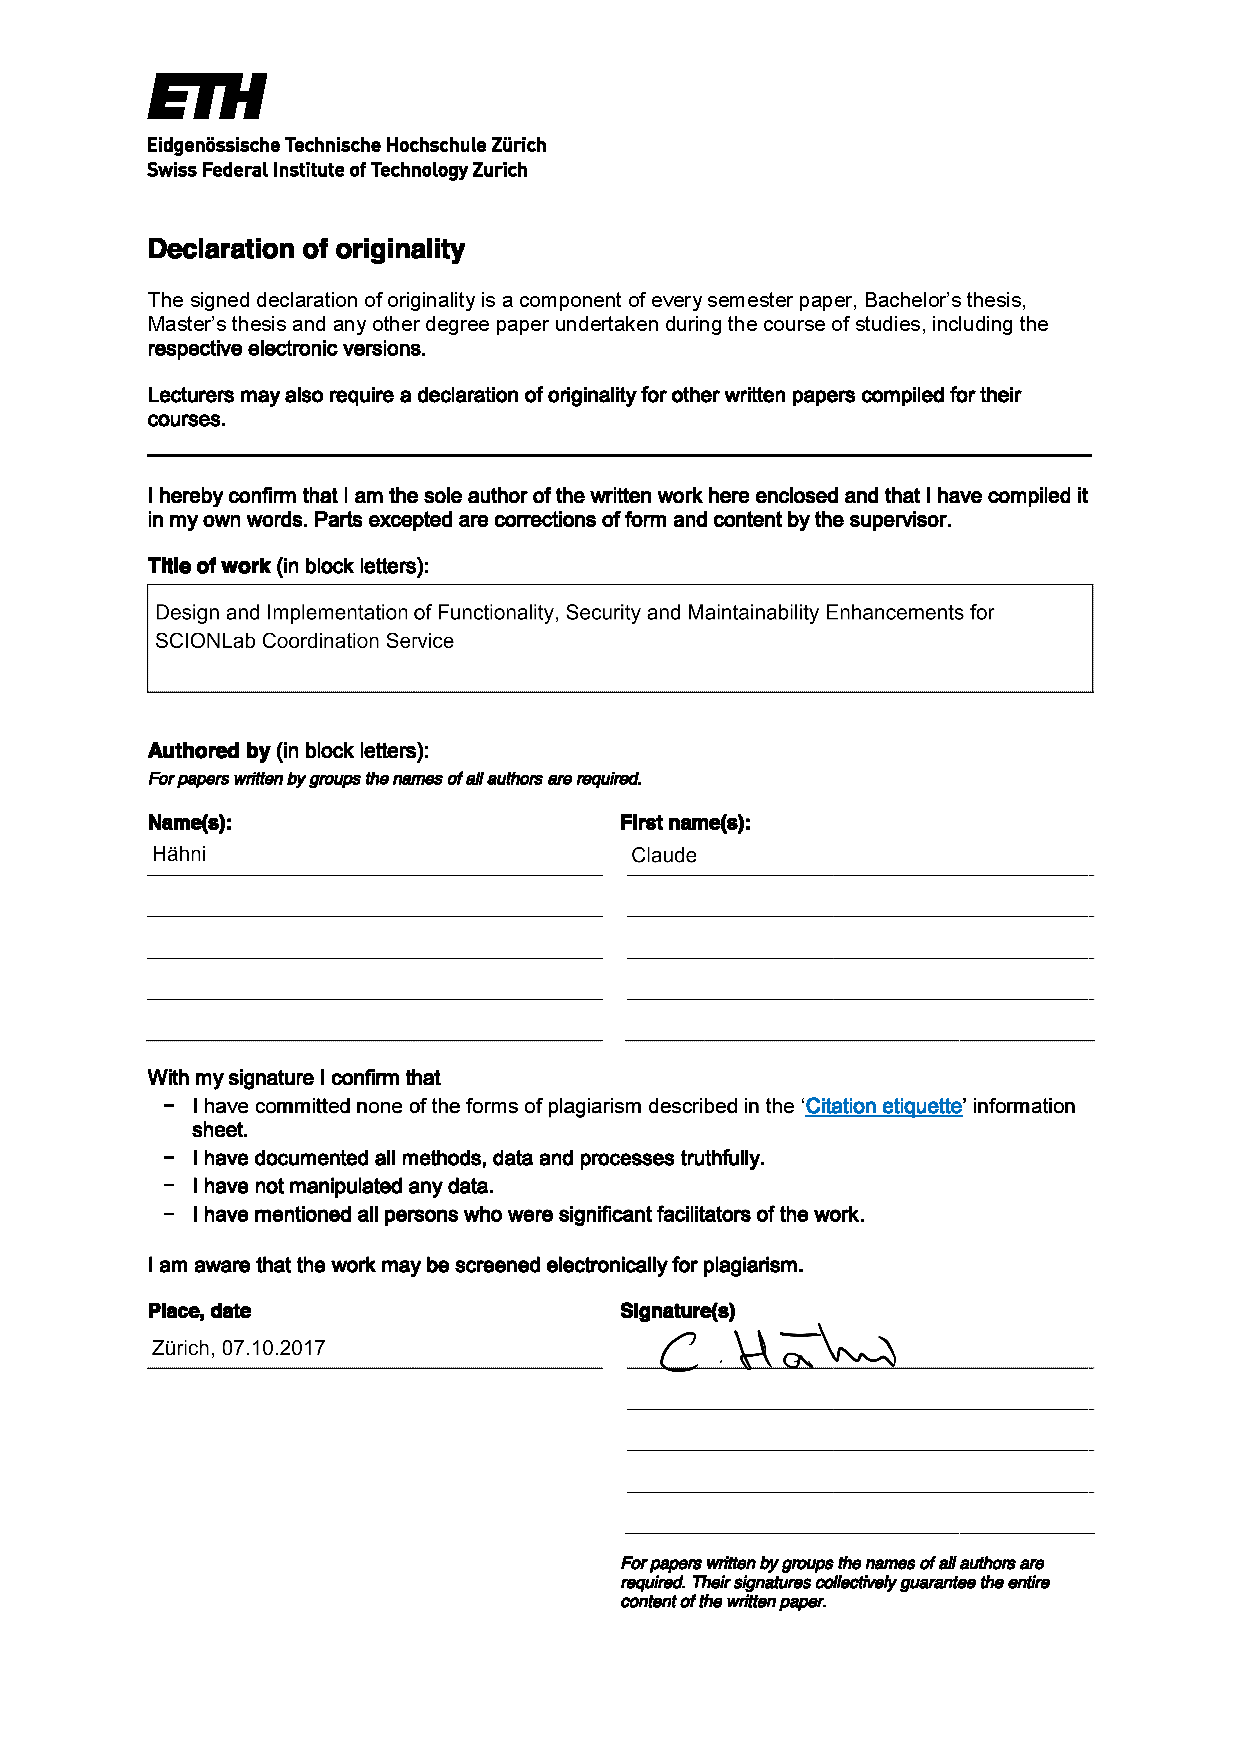
\includepdf[pages={-}]{declaration-originality-filled.pdf}

\end{document}
